\documentclass[mstat,12pt]{unswthesis}

\usepackage{color}
\usepackage{fancyvrb}
\newcommand{\VerbBar}{|}
\newcommand{\VERB}{\Verb[commandchars=\\\{\}]}
\DefineVerbatimEnvironment{Highlighting}{Verbatim}{commandchars=\\\{\}}
% Add ',fontsize=\small' for more characters per line
\usepackage{framed}
\definecolor{shadecolor}{RGB}{248,248,248}
\newenvironment{Shaded}{\begin{snugshade}}{\end{snugshade}}
\newcommand{\AlertTok}[1]{\textcolor[rgb]{0.94,0.16,0.16}{#1}}
\newcommand{\AnnotationTok}[1]{\textcolor[rgb]{0.56,0.35,0.01}{\textbf{\textit{#1}}}}
\newcommand{\AttributeTok}[1]{\textcolor[rgb]{0.13,0.29,0.53}{#1}}
\newcommand{\BaseNTok}[1]{\textcolor[rgb]{0.00,0.00,0.81}{#1}}
\newcommand{\BuiltInTok}[1]{#1}
\newcommand{\CharTok}[1]{\textcolor[rgb]{0.31,0.60,0.02}{#1}}
\newcommand{\CommentTok}[1]{\textcolor[rgb]{0.56,0.35,0.01}{\textit{#1}}}
\newcommand{\CommentVarTok}[1]{\textcolor[rgb]{0.56,0.35,0.01}{\textbf{\textit{#1}}}}
\newcommand{\ConstantTok}[1]{\textcolor[rgb]{0.56,0.35,0.01}{#1}}
\newcommand{\ControlFlowTok}[1]{\textcolor[rgb]{0.13,0.29,0.53}{\textbf{#1}}}
\newcommand{\DataTypeTok}[1]{\textcolor[rgb]{0.13,0.29,0.53}{#1}}
\newcommand{\DecValTok}[1]{\textcolor[rgb]{0.00,0.00,0.81}{#1}}
\newcommand{\DocumentationTok}[1]{\textcolor[rgb]{0.56,0.35,0.01}{\textbf{\textit{#1}}}}
\newcommand{\ErrorTok}[1]{\textcolor[rgb]{0.64,0.00,0.00}{\textbf{#1}}}
\newcommand{\ExtensionTok}[1]{#1}
\newcommand{\FloatTok}[1]{\textcolor[rgb]{0.00,0.00,0.81}{#1}}
\newcommand{\FunctionTok}[1]{\textcolor[rgb]{0.13,0.29,0.53}{\textbf{#1}}}
\newcommand{\ImportTok}[1]{#1}
\newcommand{\InformationTok}[1]{\textcolor[rgb]{0.56,0.35,0.01}{\textbf{\textit{#1}}}}
\newcommand{\KeywordTok}[1]{\textcolor[rgb]{0.13,0.29,0.53}{\textbf{#1}}}
\newcommand{\NormalTok}[1]{#1}
\newcommand{\OperatorTok}[1]{\textcolor[rgb]{0.81,0.36,0.00}{\textbf{#1}}}
\newcommand{\OtherTok}[1]{\textcolor[rgb]{0.56,0.35,0.01}{#1}}
\newcommand{\PreprocessorTok}[1]{\textcolor[rgb]{0.56,0.35,0.01}{\textit{#1}}}
\newcommand{\RegionMarkerTok}[1]{#1}
\newcommand{\SpecialCharTok}[1]{\textcolor[rgb]{0.81,0.36,0.00}{\textbf{#1}}}
\newcommand{\SpecialStringTok}[1]{\textcolor[rgb]{0.31,0.60,0.02}{#1}}
\newcommand{\StringTok}[1]{\textcolor[rgb]{0.31,0.60,0.02}{#1}}
\newcommand{\VariableTok}[1]{\textcolor[rgb]{0.00,0.00,0.00}{#1}}
\newcommand{\VerbatimStringTok}[1]{\textcolor[rgb]{0.31,0.60,0.02}{#1}}
\newcommand{\WarningTok}[1]{\textcolor[rgb]{0.56,0.35,0.01}{\textbf{\textit{#1}}}}


%%%%%%%%%%%%%%%%%%%%%%%%%%%%%%%%%%%%%%%%%%%%%%%%%%%%%%%%%%%%%%%%%%
% 
% OK...Now we get to some actual input.  The first part sets up
% the title etc that will appear on the front page
%
%%%%%%%%%%%%%%%%%%%%%%%%%%%%%%%%%%%%%%%%%%%%%%%%%%%%%%%%%%%%%%%%%

\title{Projet réalisé par\\[0.5cm] l'équipe PokéGirl du groupe de TD1 \\[3cm]Rapport
de groupe des UE \newline  Bases de données + Sciences des Données 2}

\authornameonly{Fenina Sara, Guilleminot Sarah, Rakoto Ambinintsoa
Prisca, Sbircea Stephanie. }

\author{\Authornameonly}

\copyrightfalse
\figurespagefalse
\tablespagefalse

%%%%%%%%%%%%%%%%%%%%%%%%%%%%%%%%%%%%%%%%%%%%%%%%%%%%%%%%%%%%%%%%%
%
%  And now the document begins
%  The \beforepreface and \afterpreface commands puts the
%  contents page etc in
%
%%%%%%%%%%%%%%%%%%%%%%%%%%%%%%%%%%%%%%%%%%%%%%%%%%%%%%%%%%%%%%%%%%


\input{header.tex}

\renewcommand{\contentsname}{Table des matières}

\renewcommand{\chaptername}{Chapitre}

\newcommand{\pandocbounded}[1]{#1}


\begin{document}

\beforepreface

%\afterpage{\blankpage}

% plagiarism

\prefacesection{Déclaration de non plagiat}

\vskip 2pc \noindent Nous déclarons que ce rapport est le fruit de notre seul travail, à part lorsque cela est indiqué  explicitement. 

\vskip 2pc  \noindent Nous acceptons que la personne évaluant ce rapport puisse, pour les besoins de cette évaluation:
\begin{itemize}
\item la reproduire et en fournir une copie à un autre membre de l'université; et/ou,
\item en communiquer une copie à un service en ligne de détection de plagiat (qui pourra en retenir une copie pour les besoins d'évaluation future).
\end{itemize}

\vskip 2pc \noindent Nous certifions que nous avons lu et compris les règles ci-dessus.\vspace{24pt}

\vskip 2pc \noindent En signant cette déclaration, nous acceptons ce qui précède.
\vskip 1pc \noindent
%%Signature: \rule{7cm}{0.25pt} \hfill Date: \rule{4cm}{0.25pt} \\[1cm]
%%Signature: \rule{7cm}{0.25pt} \hfill Date: \rule{4cm}{0.25pt} \\[1cm]
%%Signature: \rule{7cm}{0.25pt} \hfill Date: \rule{4cm}{0.25pt} \\[1cm]
%%Signature: \rule{7cm}{0.25pt} \hfill Date: \rule{4cm}{0.25pt} \\[1cm]
%%\vskip 1pc
Signature : Fenina Sara 
\includegraphics[width=2.3cm]{signature_saraF.png} \hfill Date : 30/03/2026 \\[0.5cm]
Signature : Guilleminot Sarah 
\includegraphics[width=2.3cm]{signature_sarahG.png} \hfill Date : 30/03/2026 \\[0cm]
Signature : Rakoto Ambinintsoa Prisca 
\includegraphics[width=4cm]{signature_prisca.png} \hfill Date : 30/03/2026 \\[0.5cm]
Signature : Sbircea Stephanie 
\includegraphics[width=2.3cm]{signature_stephanie.png} \hfill Date : 30/03/2026 \\[0.5cm]

%\textcolor{red}{Mettre à jour la date.}

{\bigskip\bigskip\noindent} \today
%\afterpage{\blankpage}

% Acknowledgements are optional


\prefacesection{Remerciements}

{\bigskip}Nous tenons à exprimer notre profonde gratitude envers les
personnes suivantes qui ont contribué à la réalisation de ce
projet.\\[1cm] Mme Sandra Bringay pour ses précieux conseils et son
soutien constant tout au long de ce projet.\\[1cm] Mme Marine Demangeot
pour son accompagnement et son aide au cours des
séances.\\[1cm] L'équipe de ce groupe pour leur collaboration et leur
dévouement, chaque membre de ce projet a apporté des idées originales et
a fait preuve de rigueur et de sérieux dans la réalisation de nos
objectifs communs.\\[1cm] 

{\bigskip\bigskip\bigskip\noindent} \today

%\afterpage{\blankpage}

% Abstract

\prefacesection{Résumé}



%\afterpage{\blankpage}


\afterpreface





%%%%%%%%%%%%%%%%%%%%%%%%%%%%%%%%%%%%%%%%%%%%%%%%%%%%%%%%%%%%%%%%%%
%
% Now we can start on the first chapter
% Within chapters we have sections, subsections and so forth
%
%%%%%%%%%%%%%%%%%%%%%%%%%%%%%%%%%%%%%%%%%%%%%%%%%%%%%%%%%%%%%%%%%%



%%%%%%%%%%%%%%%%%%%%%%%%%%%%%%%%%%%%%

%\afterpage{\blankpage}


\chapter{Introduction}\label{introduction}

Dans ce projet, nous nous intéressons au système d'échange Wonder Trade
du jeu Pokémon, dans lequel les joueurs échangent des Pokémon de manière
aléatoire avec d'autres utilisateurs à travers le monde.

La notion de qualité des échanges correspond ici à la valeur perçue des
Pokémon échangés, c'est-à-dire au niveau de satisfaction qu'ils
procurent aux joueurs. Cette qualité est appréhendée à travers plusieurs
dimensions : la puissance du Pokémon (statistiques globales), sa rareté
(shiny, légendaire), son niveau d'investissement (niveau, objets,
capacités spéciales), ainsi que le ressenti des joueurs lors de
l'échange (variable liked).

Ainsi, la problématique étudiée est la suivante :

\bigskip

\textbf{Les caractéristiques des Pokémon et des dresseurs
influencent-elles la qualité des échanges ?}

\medskip

Cette question conduit à s'interroger sur le caractère réellement
aléatoire des échanges réalisés dans le Wonder Trade du point de vue de
la qualité des Pokémon. Il s'agit notamment de déterminer si les joueurs
adoptent des comportements différenciés en échangeant davantage des
Pokémon moins performants ou moins rares, ou si des Pokémon puissants et
recherchés circulent également dans ce système. Cette analyse vise à
mettre en évidence les logiques sous-jacentes aux choix d'échange ainsi
que les stratégies potentielles des joueurs.

\medskip

Cette problématique s'inscrit à la fois dans le cadre de l'analyse de
données et de l'étude des comportements en environnement numérique. Elle
permet d'évaluer si les échanges relèvent d'une logique d'optimisation,
caractérisée par la conservation des Pokémon à forte valeur, ou s'ils
traduisent des dynamiques plus variées telles que l'aléatoire, la
générosité ou des stratégies non systématiques. L'objectif est ainsi de
caractériser les déterminants de la qualité des échanges à l'aide
d'outils statistiques.

\bigskip 
\bigskip

\medskip

\noindent

\begin{minipage}{\textwidth}
\hypertarget{uxf4les}{%
\section*{Rôles}}\label{uxf4les} % Utilisation d'une vraie section non numérotée

\textbf{Fenina Sara (22411291)}\\
Recherche des bases de données, analyse descriptive, modélisation des tables, interprétation des résultats, structuration globale.

\nopagebreak % Empêche de couper juste après
\vspace{0.3cm}

\textbf{Guilleminot Sarah (22405827)}\\
Recherche des bases de données, requêtes SQL, modélisation statistique, mise en forme du rapport, analyses et interprétations.

\nopagebreak
\vspace{0.3cm}

\textbf{Rakoto Ambinintsoa Prisca (22402951)}\\
Élaboration SQL, modélisation statistique, analyses et validation des résultats.

\nopagebreak
\vspace{0.3cm}

\textbf{Sbircea Stéphanie (22304694)}\\
Import des données, structuration base, nettoyage, transformation des données, diaporama.
\end{minipage}
\vspace{0.5cm}

\chapter{Base de données}\label{base-de-donnuxe9es}

\section{Provenance des données}\label{provenance-des-donnuxe9es}

pokemon: \url{https://www.kaggle.com/datasets/rounakbanik/pokemon}) et
wonder trades:
(\url{https://github.com/solash/pokemon-wondertrade-analytics/blob/master/data/wondertrades-03142015.json})

\bigskip

Nous avons sélectionné la table pokemon car elle contient les données
relatives à la description des Pokémon, et la table wonder trade car
elle contient les informations concernant les échanges.

Les données des Pokémons sont stockées sous format CSV : le fichier
contient 38 colonnes et 802 lignes.

Le fichier wonder trade est sous format Json, il contient 18 colonnes et
201 lignes.

\bigskip

Afin de faciliter l'analyse, nous avons choisi de filtrer certaines
colonnes. En effet, toutes les variables n'étaient pas nécessaires pour
répondre à notre problématique.

Dans la table pokemon, nous avons conservé uniquement les colonnes les
plus pertinentes, notamment celles liées aux caractéristiques
principales comme les statistiques (attack, defense, speed,
base\_total), les types (type1, type2), ainsi que des informations
générales comme la génération et le caractère légendaire.

Dans la table wonder trade, nous avons également sélectionné un
sous-ensemble de colonnes parmi les 18 colonnes initiales, pour créer
les tables trades, trainers et users comme explicité dans la partie
import des données.

\bigskip

Ce filtrage permet de réduire le nombre de variables tout en gardant les
informations essentielles, ce qui rend l'analyse plus claire et plus
pertinente.

Concernant les lignes, nous avons choisi de conserver l'ensemble des
observations, soit 802 Pokémon et 201 échanges, afin de ne pas biaiser
les résultats et de garder une vision globale des données.

\bigskip

La population étudiée correspond à l'ensemble des Pokémon du fichier
pokemon.csv ainsi qu'aux échanges du fichier wonder trade.json.

\bigskip 
\bigskip 
\medskip

\section{Descriptif des tables}\label{descriptif-des-tables}

\bigskip

La table Pokemon sert de dictionnaire de référence. Elle contient toutes
les statistiques immuables et globale de chaque espèce de Pokémon
(force, types, résistances).

\begin{longtable}{|m{3cm}|m{2cm}|m{4cm}|m{5cm}|}
\caption{Table : pokemon ($802 \times 41$)} \label{tab:pokemon} \\
\hline
\textbf{Nom colonne} & \textbf{Type} & \textbf{Signification} & \textbf{Caractéristique} \\ \hline
\endfirsthead
\hline
\textbf{Nom colonne} & \textbf{Type} & \textbf{Signification} & \textbf{Caractéristique} \\ \hline
\endhead
id\_pokemon & Entier & Identifiant interne du Pokémon & \textbf{Clé primaire} \\ \hline
pokedex\_number & Entier & Numéro officiel du Pokédex & Unique par espèce \\ \hline
name & Chaîne & Nom anglais de l'espèce & EX : Abra \\ \hline
abilities & Liste & Capacités spéciales possibles & EX : ['Overgrow'] \\ \hline
type1 / type2 & Chaîne & Types élémentaires & type2 peut être \textbf{vide} (NULL) \\ \hline

\begin{minipage}[c]{3cm}
\scriptsize\renewcommand{\arraystretch}{0.8}
\begin{tabular}{@{}l l@{}} 
hp & sp\_attack \\ 
attack & sp\_defense \\ 
defense & speed 
\end{tabular}
\end{minipage} & Entier & Statistiques de combat & 
\begin{minipage}[c]{6cm}
\scriptsize
\vspace{2mm}
- HP : $[1 ; 255]$  \\
- Attaque : $[5 ; 190]$  \\
- Défense : $[5 ; 230]$ \\
- Att. Spé : $[10 ; 216]$  \\
- Déf. Spé : $[20 ; 230]$  \\
- Vitesse : $[5 ; 200]$ 
\vspace{2mm}
\end{minipage} \\ \hline


base\_total & Entier & Somme des statistiques AKA Puissance globale & base\_total : $[180 ; 780]$  \\ \hline
is\_legendary & Booléen & Statut de Pokémon légendaire & 0 = Non, 1 = Oui \\ \hline
resistance & Réel & Multiplicateurs de dégâts & resistance : $[0 ; 36]$  \\ \hline


\end{longtable}

\smallskip
\bigskip

\begin{longtable}{|p{3cm}|p{2cm}|p{4cm}|p{5cm}|}
\caption{Table : trades} \label{tab:trades} \\
\hline
\textbf{Nom colonne} & \textbf{Type} & \textbf{Signification} & \textbf{Caractéristique} \\ \hline
\endfirsthead
\hline
\textbf{Nom colonne} & \textbf{Type} & \textbf{Signification} & \textbf{Caractéristique} \\ \hline
\endhead
pokemonId & Entier & ID du Pokémon échangé & \textbf{Clé étrangère} vers pokemon \\ \hline
trainerId & Entier & ID du dresseur partenaire & \textbf{Clé étrangère} vers trainers \\ \hline
userId & Entier & ID de l'utilisateur local & \textbf{Clé étrangère} vers users \\ \hline
level & Entier & Niveau du Pokémon lors de l'échange &$ level : [0 ;100]$  \\ \hline
isShiny & Texte & Aspect chromatique rare & "VRAI" ou "FAUX" \\ \hline
hasItem & Texte & Le Pokémon tient-il un objet ? & "VRAI" ou "FAUX" \\ \hline
hasHiddenAbility & Texte & Possède un talent caché rare & "VRAI" ou "FAUX" \\ \hline
hasPerfectIV & Texte & Possède des stats innées au max & "VRAI" ou "FAUX" \\ \hline
hasPokerus & Texte & Infecté par le virus bénéfique & "VRAI" ou "FAUX" \\ \hline
hasEggMove & Texte & Possède une capacité de reproduction & "VRAI" ou "FAUX" \\ \hline
liked & Chaîne & Avis de l'utilisateur sur l'échange & "like", "dislike" ou \textbf{vide} \\ \hline
date / time & Date / Heure & Moment précis de l'échange & EX : 2015-02-08 / 54817 \\ \hline
\end{longtable}

\smallskip

La table Trades est centrale. Elle enregistre l'historique de tous les
échanges effectués. Contrairement à la table précédente, les données ici
(niveau, objet, shiny) sont spécifiques au spécimen précis qui a été
reçu lors de l'échange.

\smallskip

\begin{longtable}{|p{3cm}|p{2cm}|p{4cm}|p{5cm}|}
\caption{Table : trainers} \label{tab:trainers} \\
\hline
\textbf{Nom colonne} & \textbf{Type} & \textbf{Signification} & \textbf{Caractéristique} \\ \hline
\endfirsthead
\hline
\textbf{Nom colonne} & \textbf{Type} & \textbf{Signification} & \textbf{Caractéristique} \\ \hline
\endhead
id\_trainer & Entier & Identifiant unique du dresseur & \textbf{Clé primaire} \\ \hline
trainer\_name & Chaîne & Pseudo du dresseur & Peut être \textbf{vide} (si anonyme) \\ \hline
gender & Chaîne & Sexe du dresseur & "male" ou "female" \\ \hline
country & Chaîne & Code pays (ISO) & EX : US, JP, FR \\ \hline
country\_sub1 & Chaîne & Région ou État d'origine & EX : California, Texas, Tokyo \\ \hline
\end{longtable}

\smallskip

La table Trainers contient les profils des partenaires d'échange. Elle
permet de savoir avec qui l'utilisateur a interagi et de quelle région
du monde provient le Pokémon reçu. \smallskip

\begin{longtable}{|p{3cm}|p{2cm}|p{4cm}|p{5cm}|}
\caption{Table : users} \label{tab:users} \\
\hline
\textbf{Nom colonne} & \textbf{Type} & \textbf{Signification} & \textbf{Caractéristique} \\ \hline
\endfirsthead
\hline
\textbf{Nom colonne} & \textbf{Type} & \textbf{Signification} & \textbf{Caractéristique} \\ \hline
\endhead
id\_user & Entier & Identifiant unique de l'utilisateur & \textbf{Clé primaire} \\ \hline
\end{longtable}
\smallskip

La table Users est très courte et sert simplement à identifier les
comptes locaux sur le logiciel du site web qui a enregistré les données.
\smallskip

\section{Modèles MCD et MOD}\label{moduxe8les-mcd-et-mod}

\subsection{MCD}\label{mcd}

\begin{figure}
\centering
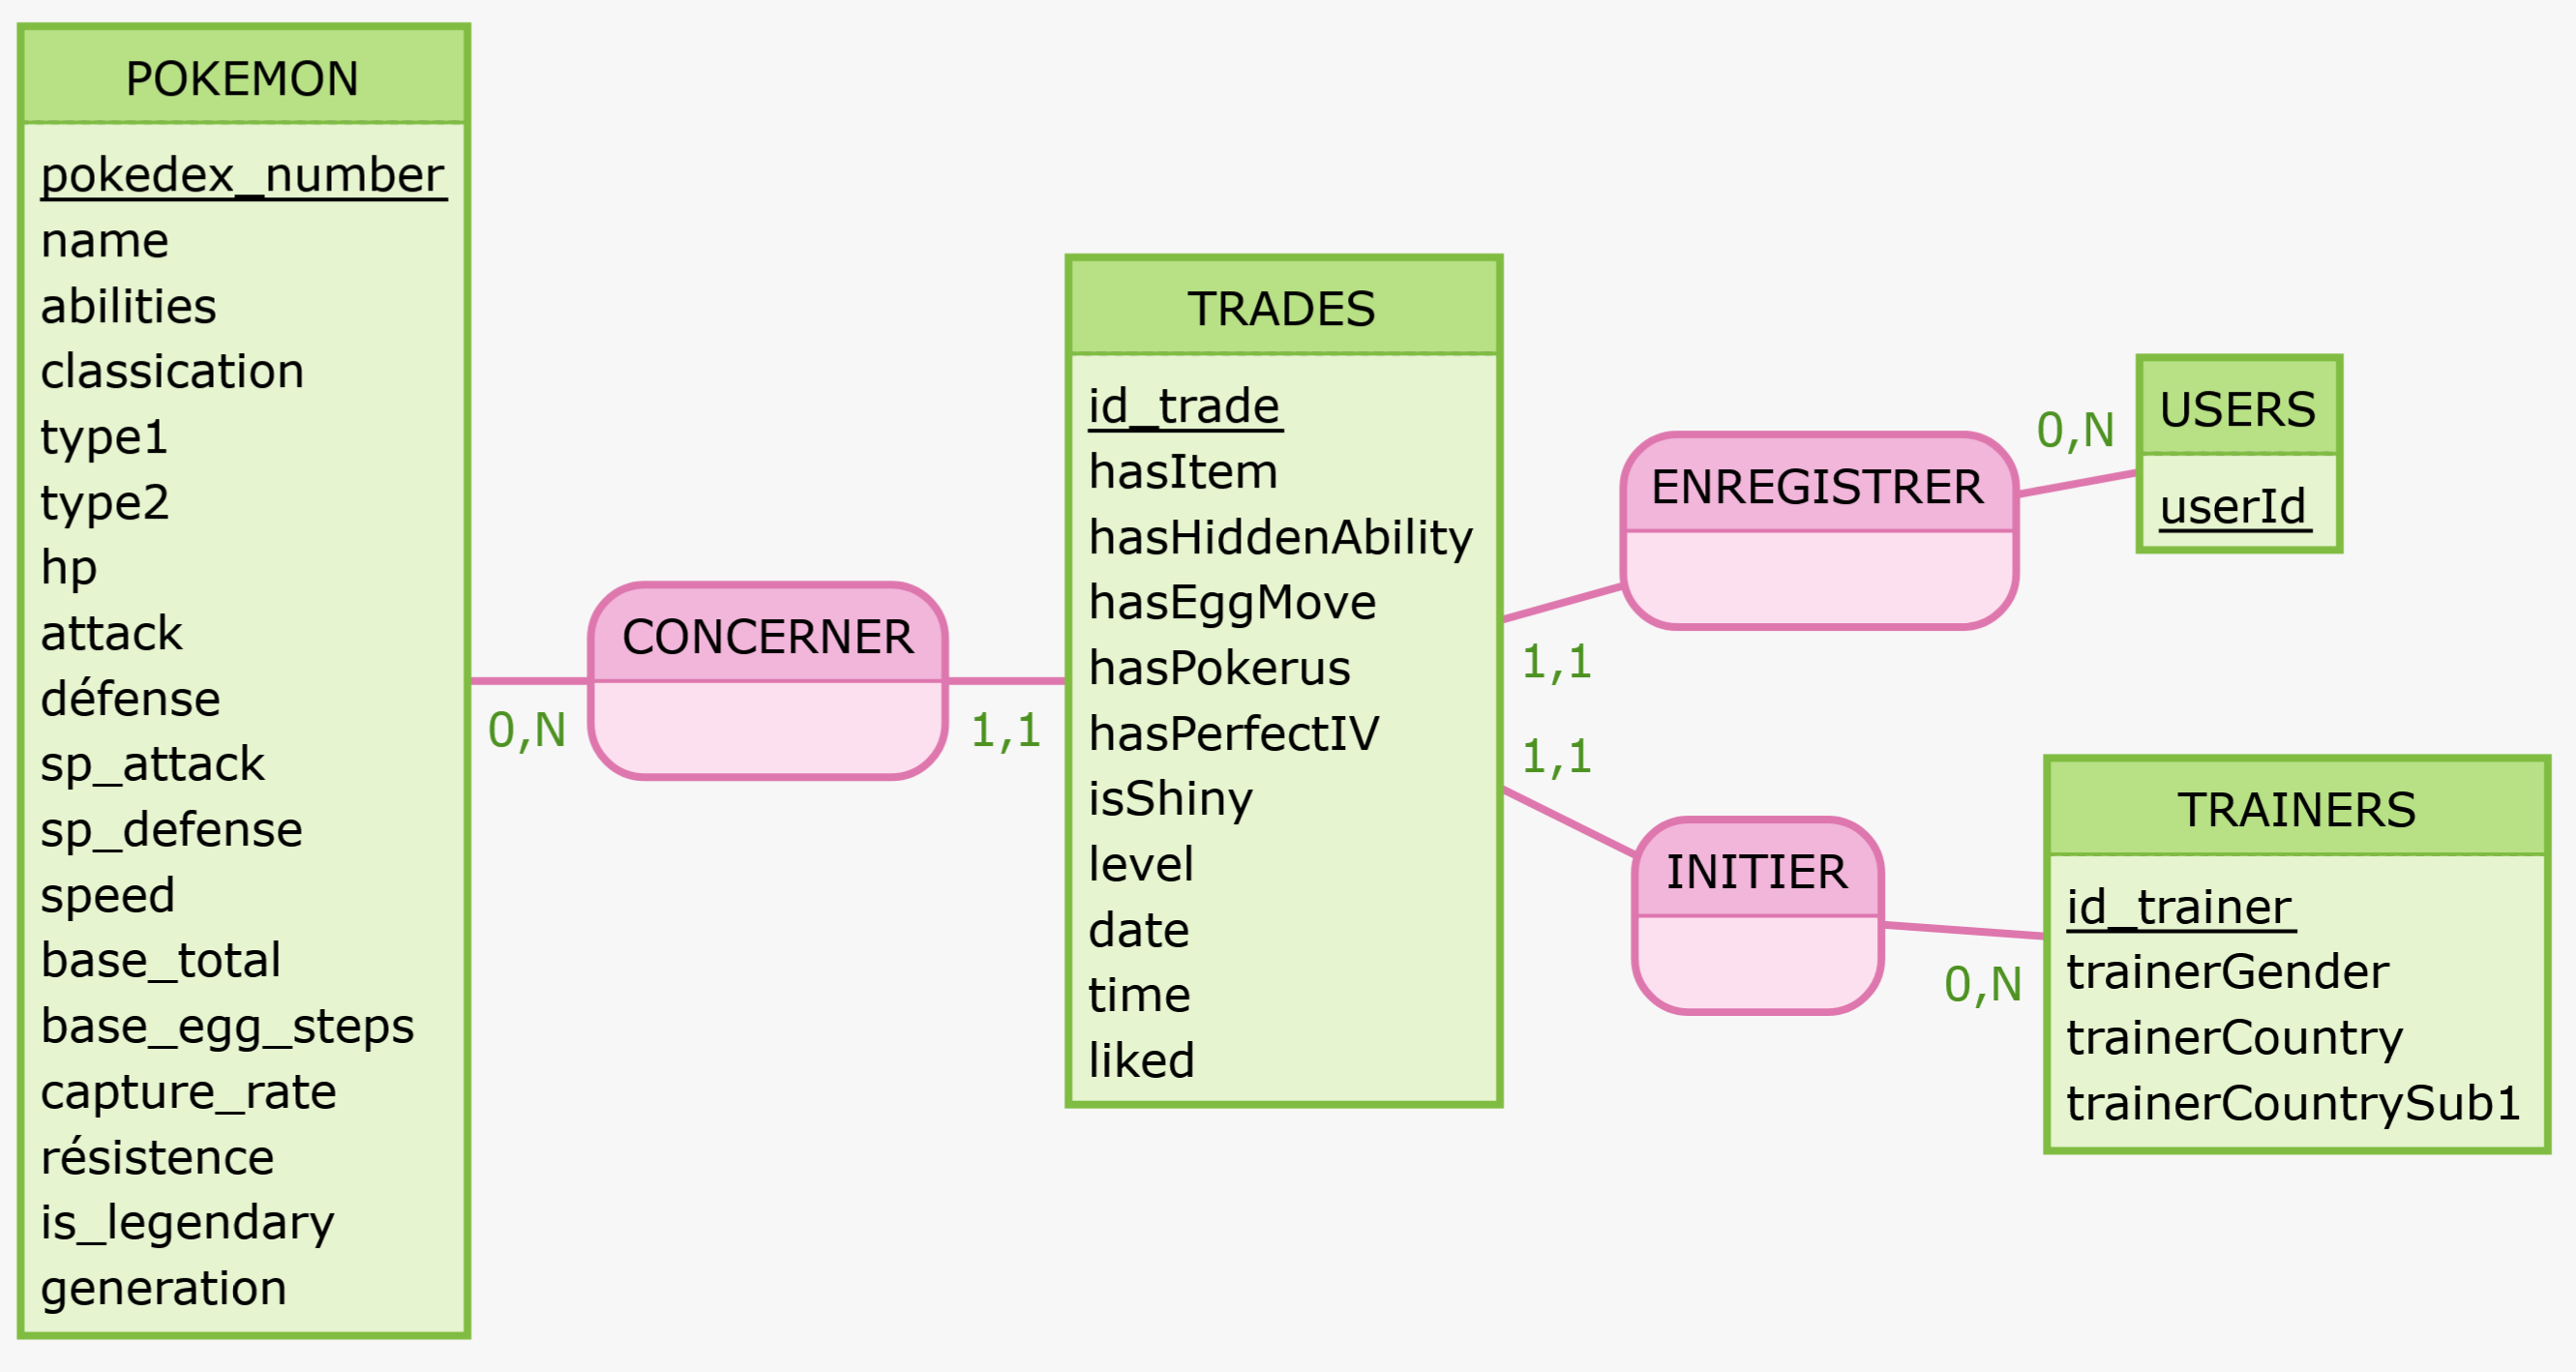
\includegraphics[width=16cm,height=\textheight,keepaspectratio,alt={MCD.}]{tuto-0019(1).png}
\caption{\textbf{MCD}.}\label{MCD}
\end{figure}

\smallskip

\subsection{MOD :}\label{mod}

\begin{figure}
\centering
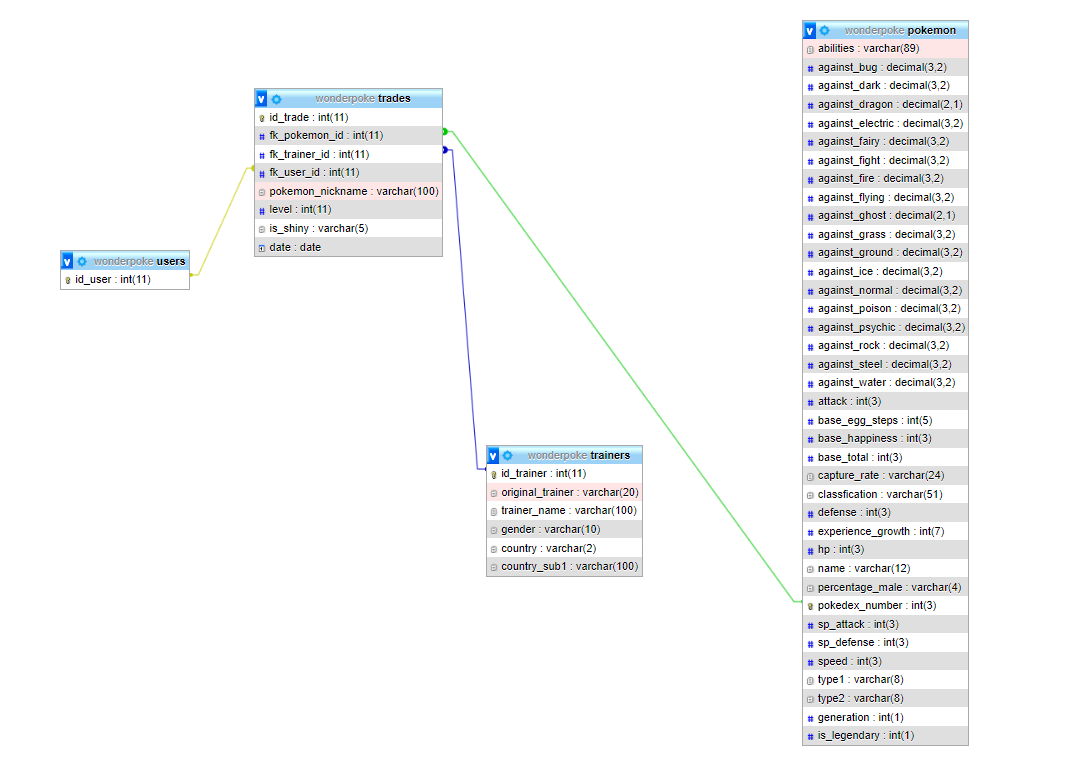
\includegraphics[width=16cm,height=8cm,alt={** MOD.**}]{pokewonder (1).png}
\caption{** MOD.**}\label{MOD}
\end{figure}

\bigskip 
\bigskip 
\bigskip 
\bigskip

MOD :

\textbf{USERS} (id\_user)

\textbf{TRAINER} (id\_trainer, original\_trainer\_id, trainer\_name,
gender, country, country\_sub1)

\textbf{POKEMON} (pokedex\_number, name, abilities, classication, type1,
type2, hp, attack, défense, sp\_attack, sp\_defense, speed, base\_total,
base\_egg\_steps, percentage\_male, capture\_rate, résistence,
is\_legendary, generation)

\textbf{TRADE} (id\_trade, hasItem, hasHiddenAbility,
hasEggMove,hasPokerus, hasPerfectIV, isShiny, level, date, time, liked,
\#id\_user, \#id\_trainer, \#pokedex\_number)

\bigskip 
\bigskip

\section{Import des données}\label{import-des-donnuxe9es}

A partir des fichiers \textbf{Pokemon} et \textbf{WonderTrade}, nous
avons créé les tables \textbf{Pokemon}, \textbf{Trades},
\textbf{Trainers} et \textbf{Users} comme indiqué si-dessous.

\bigskip

\subsection{Transformation du fichier Json en csv
:}\label{transformation-du-fichier-json-en-csv}

Nous avons importé le fichier \textbf{WonderTrade} qui est en Json sur
Excel en allant sur ``obtenir des données'' puis ``à partir d'un
fichier'' puis ``à partir de JSON'' comme le montre la Figure.1, ce qui
nous a permi de le convertir en table avec l'éditeur Power Query.

\bigskip

Nous avons choisi de garder toutes les colonnes en cliquant sur la
double flèche et en sélectionnant le tout comme le montre la Figure.3,
puis nous avons pu avoir le fichier en csv grâce au bouton ``fermer et
charger''.

\subsection{Création des nouveaux Trainer ID
:}\label{cruxe9ation-des-nouveaux-trainer-id}

Directement dans le fichier CSV \textbf{WonderTrade} ouvert dans
LibreOffice, nous avons procédé de la manière suivante :

\bigskip

Nous avons d'abord activé l'autofiltre sur l'ensemble des données afin
de faciliter les opérations de tri, pour ensuite trier par ordre
croissant \textbf{\emph{trainerGender}} puis
\textbf{\emph{TrainerCountry}} puis \textbf{\emph{TrainerCountrySub1}}.

\bigskip

Ce tri permet de regrouper les lignes présentant des caractéristiques
similaires, ce qui est nécessaire pour la suite du traitement.

\bigskip

Nous avons ensuite trié la colonne \textbf{\emph{trainerId}} par ordre
croissant. Nous avons constaté que les lignes situées en bas du tableau
correspondent aux échanges avec un trainerId vide. Ce sont ces lignes
pour lesquelles nous devons créer de nouveaux identifiants.

\bigskip

Nous faisons ici l'hypothèse que des individus ayant le même genre, le
même pays et la même sous-localisation correspond à une seule et même
personne. Sachant qu'il y a environ 100 lignes sans ID et que les
identifiants existants commencent à 783, il n'y aura pas de problème
pour créer les nouveaux.

\bigskip

Sous le dernier \textbf{\emph{trainerId}} connu, nous saisissons la
valeur 1, puis dans la cellule suivante, nous entrons la formule :

\bigskip

\begin{verbatim}
  “=SI(J103=J104;SI(K103=K104;SI(L103=L104;Q103;Q103+1);Q103+1);Q103+1)”
\end{verbatim}

\bigskip

Nous étirons ensuite cette formule jusqu'à la dernière ligne du tableau.

\bigskip

Cette formule permet de comparer chaque ligne à la précédente : si le
genre, le pays et la sous-localisation sont identiques, l'identifiant
reste le même ; dans le cas contraire, il est incrémenté de 1.

\bigskip

Nous avons choisi cette méthode en considérant que les trainers
partageant les mêmes caractéristiques correspondent à une seule
personne. Il aurait également été possible d'attribuer un identifiant
distinct à chaque trainer anonyme, mais ce choix n'a pas d'impact sur
notre analyse, qui porte sur les caractéristiques des individus (genre,
pays, etc.) et non sur leur identification individuelle.

\bigskip

\subsection{Création des tables dérivées de WonderTrade
:}\label{cruxe9ation-des-tables-duxe9rivuxe9es-de-wondertrade}

À partir du fichier \textbf{WonderTrade} modifié, nous avons construit
plusieurs tables :

\bigskip

\begin{figure}
\centering
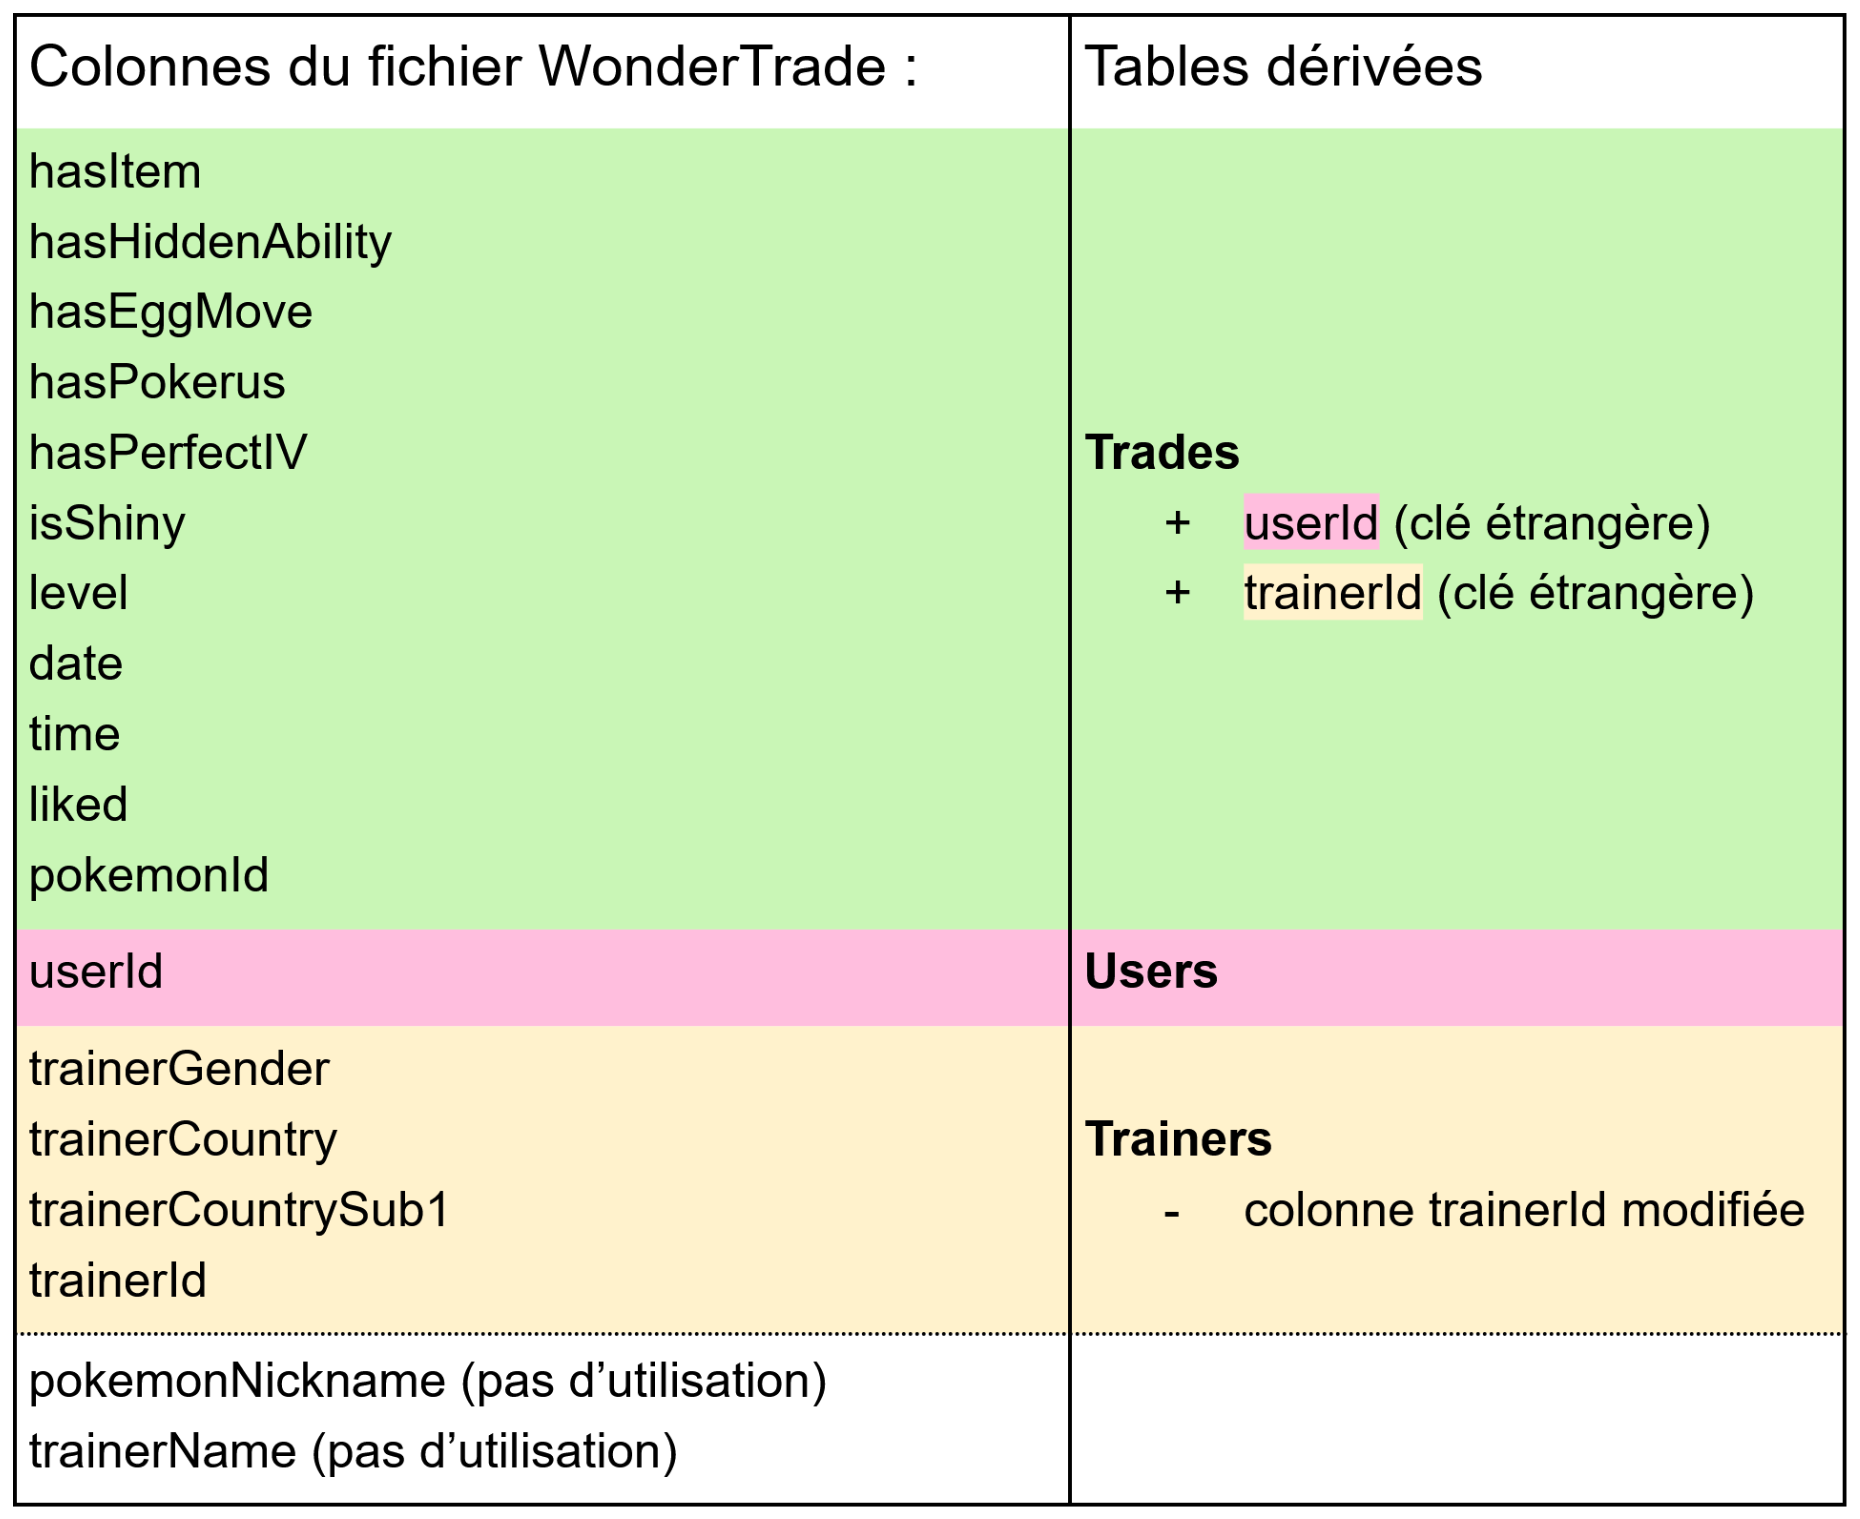
\includegraphics[width=12cm,height=\textheight,keepaspectratio,alt={Schéma explication tables dérivées wondertrade.}]{schema_wondertrade.png}
\caption{\textbf{Schéma explication tables dérivées
wondertrade.}}\label{MOD}
\end{figure}

Ce découpage suit rigoureusement les règles de passage du MCD au MOD
pour garantir la normalisation de la base de données. Eviter de répéter
inutilement les informations. Par exemple, les caractéristiques d'un
dresseur (pays, genre) ne sont enregistrées qu'une seule fois dans la
table Trainers, même s'il effectue des dizaines d'échanges. Chaque
entité distincte identifiée dans notre analyse a été transformée en
table indépendante : Users, Trainers et Trades. Pour maintenir les liens
relationnels, les identifiants userId et id\_trainer ont été intégrés à
la table centrale Trades en tant que clés étrangères (\#id\_user,
\#id\_trainer).

Cette structure relationnelle est indispensable pour réaliser des
jointures SQL optimisées et mener les analyses statistiques (ANOVA,
Khi²) demandées sans biais de répétition

\bigskip

\subsection{Dernières modifications :}\label{derniuxe8res-modifications}

Table \textbf{Pokemon} : Nous avons ouvert le fichier CSV pokemon avec
LibreOffice afin de supprimer les colonnes inutiles :
\textbf{\emph{weight\_kg, japanese\_name, height\_m, experience\_growth,
base\_happiness}}.

\bigskip

Pour diminuer les colonnes en gardant les données de résistance
nécessaire, nous commençons par rechercher et remplacer les ``.'' par
des ``,'' pour que les réels soient bien tous considérés comme des
nombres par LibreOffice.

\bigskip

Ensuite nous créons une nouvelle colonne \textbf{\emph{résistance}} avec
le code ``=SOMME(B2:S2)'' donc la somme de toutes les colonnes
commençant par \textbf{\emph{against}}, que nous étirons jusqu'à la
dernière ligne. Puis nous faisons un copié collé de cette colonne
\textbf{\emph{résistance}} au même endroit en texte non formaté avec un
séparateur qui n'est pas '',''afin de conserver les données après avoir
supprimé les autres colonnes, et enfin dernier nous pouvons supprimer
toutes les colonnes \textbf{\emph{against\ldots{}}}.

\bigskip

Tables \textbf{Trainers} et \textbf{Users} : Nous avons ouvert ces
tables dans LibreOffice, puis nous avons trié les données par
identifiant croissant, et enfin nous avons ensuite supprimé manuellement
les lignes en double.

\bigskip

Table \textbf{Trades} : Afin de simplifier l'analyse future, dans
LibreOffice nous faisons un copié-collé des noms de colonnes
\textbf{\emph{hasItem, hasHiddenAbility, hasEggMove, hasPokerus,
hasPerfectIV et isShiny}} à droite des autres colonnes. Nous écrivons
ensuite le code ``=SI(B2=``FAUX'';0;1)'' dans la case sous
\textbf{\emph{hasItem}} que nous étirons jusqu'à la dernière case du
nouveau \textbf{\emph{isShiny}}. Comme précédemment nous copions et
collons en texte non formaté et supprimons les colonnes de trop.

\bigskip

Nous ajoutons ensuite une clé primaire auto-incrémentée dans phpMyAdmin
en utilisant la requête SQL suivante :

\bigskip

\begin{verbatim}
  “ALTER TABLE trades ADD IdTrade INT AUTO_INCREMENT PRIMARY KEY;”
\end{verbatim}

\bigskip 
\bigskip

\chapter{Requêtes réalisées}\label{requuxeates-ruxe9alisuxe9es}

\begin{verbatim}
## Warning: le package 'DBI' a été compilé avec la version R 4.5.3
\end{verbatim}

REQUETE N.0: Pokémon échangés vs non échangés

\bigskip

Pour commencer, nous avons interrogé le logiciel pour connaître le
nombre de pokémon échangé vs le nombre de pokémon jamais échangé. Ces
deux premières requêtes vont être à l'origine des autres requêtes qui
vous surtout se concentrer sur les pokémons échangés.

\begin{Shaded}
\begin{Highlighting}[]
\KeywordTok{SELECT} 
    \FunctionTok{COUNT}\NormalTok{(}\KeywordTok{DISTINCT}\NormalTok{ t.pokemonId) }\KeywordTok{AS}\NormalTok{ nb\_pokemon\_echanges,}
\NormalTok{    (}\KeywordTok{SELECT} \FunctionTok{COUNT}\NormalTok{(}\OperatorTok{*}\NormalTok{) }\KeywordTok{FROM}\NormalTok{ Pokemon) }\OperatorTok{{-}} \FunctionTok{COUNT}\NormalTok{(}\KeywordTok{DISTINCT}\NormalTok{ t.pokemonId)}
    \KeywordTok{AS}\NormalTok{ nb\_pokemon\_non\_echanges}
\KeywordTok{FROM}\NormalTok{ Pokemon p}
\KeywordTok{LEFT} \KeywordTok{JOIN}\NormalTok{ Trades t }\KeywordTok{ON}\NormalTok{ p.pokedex\_number }\OperatorTok{=}\NormalTok{ t.pokemonId;}
\end{Highlighting}
\end{Shaded}

\begin{longtable}[]{@{}rr@{}}
\caption{1 records}\tabularnewline
\toprule\noalign{}
nb\_pokemon\_echanges & nb\_pokemon\_non\_echanges \\
\midrule\noalign{}
\endfirsthead
\toprule\noalign{}
nb\_pokemon\_echanges & nb\_pokemon\_non\_echanges \\
\midrule\noalign{}
\endhead
\bottomrule\noalign{}
\endlastfoot
119 & 682 \\
\end{longtable}

On observe que tous les Pokémon ne sont pas échangés, ce qui montre que
certains sont conservés par les joueurs. Cela suggère que les décisions
d'échange ne sont pas aléatoires mais dépendent de certaines
caractéristiques.

****préciser qu'il y a seulement 200 echanges pour environ 800 pokémons
en tout donc plutot dire qu'il y a des répétitions, qu'on va peut etre
analyser par la suite, préciser qu'avec 800 échanges on serait donc à
peu près sure d'avoir une certaine quantité de pokémons jamais
échangés****

\bigskip

REQUETE N.1: Pokémon de niveau 1(breeding)

\bigskip

Nous cherchons à savoir combien de Pokémon échangés sont de niveau 1, ce
qui correspond souvent à des Pokémon issus d'élevage.

\begin{Shaded}
\begin{Highlighting}[]
\KeywordTok{SELECT} \FunctionTok{COUNT}\NormalTok{(}\OperatorTok{*}\NormalTok{) }\KeywordTok{AS}\NormalTok{ nb\_pokemon\_niveau1}
\KeywordTok{FROM}\NormalTok{ trades}
\KeywordTok{WHERE} \KeywordTok{level} \OperatorTok{=} \DecValTok{1}\NormalTok{;}
\end{Highlighting}
\end{Shaded}

\begin{longtable}[]{@{}r@{}}
\caption{1 records}\tabularnewline
\toprule\noalign{}
nb\_pokemon\_niveau1 \\
\midrule\noalign{}
\endfirsthead
\toprule\noalign{}
nb\_pokemon\_niveau1 \\
\midrule\noalign{}
\endhead
\bottomrule\noalign{}
\endlastfoot
72 \\
\end{longtable}

Un grand nombre de Pokémon sont de niveau 1. Cela montre que les joueurs
pratiquent le breeding et échangent les Pokémon non optimaux.
****préciser que ça revient à un peu plus d'1/3, alors que le niveau le
plus haut présent est 74 donc si c'était partagé équitablement 1/73
-\textgreater{} c'est pour ça qu'on peut dire qu'il est beaucoup plus
présent****

\bigskip

REQUETE N.2: HP échangés vs non échangés

\bigskip

Nous avons ensuite comparé les points de vie moyens (HP) des Pokémon
échangés et non échangés.

L'objectif est de déterminer si les dresseurs ont tendance à échanger
des Pokémon plus faibles, plus forts ou équivalents à la moyenne.

\begin{figure}
\centering
\includegraphics[width=10cm,height=4cm,alt={Requête 2.}]{requete1.png}
\caption{\textbf{Requête 2}.}\label{requete1}
\end{figure}

Si les Pokémon échangés ont en moyenne moins de HP, cela suggère que les
joueurs échangent plutôt des Pokémon plus faibles. À l'inverse, une
moyenne similaire indiquerait que le HP n'est pas un critère déterminant
dans les échanges.

\bigskip

REQUETE N.3: Genre du dresseur et type de Pokémon

\bigskip

Nous avons étudié le lien entre le genre des dresseurs et les types de
Pokémon échangés.

L'objectif est de vérifier s'il existe une corrélation entre le genre et
ses préférences d'échange.

Cette requête permet de révéler des préférences de types (ex : feu, eau,
normal\ldots) ou l'absence totale de différence (comportement homogène).
Cela permet d'introduire une dimension sociologique dans l'analyse.

\begin{figure}
\centering
\includegraphics[width=15cm,height=6cm,alt={Requête 3.}]{requete3.png}
\caption{\textbf{Requête 3}.}\label{requete3}
\end{figure}

Les résultats permettent d'observer s'il existe une différence de
comportement entre les dresseurs selon leur genre. Toutefois, toute
différence observée doit être interprétée avec prudence, car elle peut
être faible ou non significative.

\bigskip

REQUETE N.4: Types les moins appréciés

\bigskip

Puis nous avons analysé les types des Pokémons dans les détails pour
étudier lesquels sont les moins appréciés.

\begin{figure}
\centering
\includegraphics[width=10cm,height=4cm,alt={Requête 4.}]{requete4.png}
\caption{\textbf{Requête 4}.}\label{requete4}
\end{figure}

Le type Normal est le moins aimé car il regroupe les Pokémon les plus
communs et faciles à capturer dès le début du jeu. Statistiquement, ils
possèdent souvent des caractéristiques de combat plus faibles (HP,
Attaque, Défense) que les types plus rares ou ``exotiques''. Enfin,
comme les dresseurs utilisent souvent le Wonder Trade comme un outil
d'optimisation pour se débarrasser de leurs spécimens les plus faibles,
le système se retrouve saturé de Pokémon de type Normal, provoquant une
déception systématique enregistrée dans la colonne liked (dislike) par
les destinataires

\bigskip

REQUETE N.5: Shiny

\bigskip

Nous avons cherché à identifier les Pokémon shiny présents dans les
échanges.

L'objectif est d'évaluer si les Pokémon rares sont fréquemment échangés.

\begin{figure}
\centering
\includegraphics[width=10cm,height=4cm,alt={Requête 5.}]{requete5.png}
\caption{\textbf{Requête 5}.}\label{requete5}
\end{figure}

Interprétation : Les résultats montrent qu'ils sont très peu échangés,
ce qui est logique car :

ils sont rares ils ont une forte valeur pour les joueurs

Cela confirme un comportement de rétention des ressources rares.

\bigskip

REQUETE N.6 : Niveau moyen

\bigskip

Nous avons calculé le niveau moyen des Pokémon échangés. L'objectif est
de mesurer le niveau global des échanges.Plus le niveau est élevé plus
l''échange est stratégique et plus il est faible plus l'échange est
commun.

\begin{figure}
\centering
\includegraphics[width=10cm,height=4cm,alt={Requête 6.}]{requete6.png}
\caption{\textbf{Requête 6}.}\label{requete6}
\end{figure}

Le niveau moyen des Pokémon échangés permet d'évaluer la qualité globale
des échanges. Un niveau relativement faible suggère que les joueurs
échangent principalement des Pokémon peu stratégiques, tandis que les
Pokémon de haut niveau sont davantage conservés.

\bigskip

REQUETE N.7: Egg Move et HP

\bigskip

Nous avons analysé si la présence d'une capacité spéciale (Egg Move)
influence les HP moyens afin de voir si cette caractéristique apporte un
avantage mesurable.

\begin{figure}
\centering
\includegraphics[width=10cm,height=4cm,alt={Requête 7.}]{requete7.png}
\caption{\textbf{Requête 7}.}\label{requete7}
\end{figure}

Les résultats permettent de comparer les HP moyens selon la présence
d'Egg Moves. Si la différence est faible, cela suggère que cette
caractéristique n'a pas d'impact significatif sur les performances
globales des Pokémon échangés.

\bigskip

Requête N.8 : Anonymat vs qualité

\bigskip

NB : Nous avons eu recours à une IA pour formuler cette requête.

Nous avons comparé les échanges entre dresseurs anonymes et identifiés à
partir de plusieurs indicateurs (niveau, shiny, objets, IV\ldots).

L'objectif est de mesurer si l'anonymat influence la qualité des
échanges.Elle permet de vérifier si les joueurs anonymes proposent des
échanges moins intéressants ou si aucune différence significative
n'existe

En revanche La qualité est multidimensionnelle, donc une analyse SQL
seule ne suffit pas. Il faudrait pondérer les variables pour créer un
score global.

\begin{figure}
\centering
\includegraphics[width=16cm,height=8cm,alt={Requête 8.}]{requete8.png}
\caption{\textbf{Requête 8}.}\label{requete8}
\end{figure}

REQUETE N.9: Dresseur le plus actif

\bigskip

Cette requête permet d'observer le comportement du dresseur le plus
actif. Cependant, elle constitue une analyse de cas particulier et ne
permet pas de généraliser à l'ensemble des joueurs.

Nous avons identifié le niveau maximal du Pokémon appartenant au
dresseur ayant effectué le plus d'échanges.

L'objectif est de relier activité (nombre d'échanges) et performance
(niveau du Pokémon)

\begin{figure}
\centering
\includegraphics[width=10cm,height=4cm,alt={Requête 9.}]{requete9.png}
\caption{\textbf{Requête 9}.}\label{requete}
\end{figure}

Requête N.10 : Relation entre la facilité de capture et le nombre
d'échanges

\bigskip

Nous avons étudié la relation entre la facilité de capture et le nombre
d'échanges. L'objectif est de tester si les Pokémon faciles à capturer
sont plus échangés.

\begin{figure}
\centering
\includegraphics[width=10cm,height=8cm,alt={Requête 10.}]{requete10.png}
\caption{\textbf{Requête 10}.}\label{requete10}
\end{figure}

Les résultats permettent d'analyser la relation entre la rareté des
Pokémon et leur fréquence d'échange. Une forte présence de Pokémon
faciles à capturer dans les échanges indiquerait que les joueurs
privilégient l'échange de Pokémon communs, tandis que les Pokémon rares
sont conservés.

\bigskip
\bigskip

\#\#Conclusion générale

L'ensemble des analyses réalisées sur les échanges Wonder Trade met en
évidence que les échanges ne sont pas totalement aléatoires.

Plusieurs facteurs semblent influencer les décisions des joueurs,
notamment les caractéristiques des Pokémon et leur niveau de
performance. Les résultats montrent que les Pokémon échangés sont
fréquemment de niveau faible ou intermédiaire, ce qui suggère une
tendance des joueurs à se séparer des Pokémon les moins optimisés.

Par ailleurs, les analyses liées à la rareté (comme les Pokémon shiny ou
la facilité de capture) indiquent que les Pokémon les plus rares ou
difficiles à obtenir sont moins souvent échangés, confirmant un
comportement de conservation des ressources précieuses par les joueurs.

Enfin, l'étude des profils de dresseurs montre que certains
comportements peuvent varier selon les caractéristiques des
utilisateurs, mais ces différences restent globalement modérées.

Dans l'ensemble, ces résultats suggèrent que les échanges Wonder Trade
sont influencés par une logique d'optimisation des joueurs, plutôt que
purement aléatoire : les Pokémon jugés faibles ou communs sont davantage
échangés, tandis que les Pokémon rares ou performants sont
majoritairement conservés.

\section{Quelques détails
techniques}\label{quelques-duxe9tails-techniques}

\chapter{Modélisation statistique}\label{moduxe9lisation-statistique}

L'objectif de cette analyse est de déterminer si les caractéristiques
des Pokémon et des dresseurs influencent la qualité des échanges dans le
système de Wonder Trade.

La qualité d'un échange est mesurée à l'aide de la variable liked, qui
traduit le ressenti du joueur (échange apprécié ou non).

Nous analysons deux dimensions :

Les caractéristiques intrinsèques du Pokémon : rareté (shiny),
puissance, facilité de capture Les caractéristiques liées au dresseur :
comportement et investissement (niveau)

Afin de répondre à cette problématique, nous mobilisons plusieurs outils
statistiques : le test du Khi², l'analyse de variance (ANOVA) et un test
de corrélation.

\emph{I. Influence de la rareté sur la satisfaction (Test du Khi²)}

\subsection{Objectif}\label{objectif}

Lorsque nous comparons les effectifs de Pokémon échangés selon leur
rareté (par exemple shiny ou non shiny), nous remarquons que certaines
catégories sont très peu représentées par rapport à d'autres. Cela peut
laisser penser que les échanges ne sont pas totalement aléatoires, mais
influencés par le comportement des joueurs. Nous allons donc vérifier si
la répartition des Pokémon échangés est indépendante de leur rareté en
utilisant un test du Khi².

Lorsque nous observons la répartition des Pokémon échangés, certaines
catégories, notamment les Pokémon rares, apparaissent moins fréquentes.
Cela suggère que les échanges pourraient ne pas être totalement
aléatoires, mais influencés par des choix stratégiques des joueurs. Nous
cherchons donc à déterminer si le fait qu'un Pokémon soit shiny
influence la satisfaction des joueurs (liked). Hypothèses statistisques

H0 (Hypothèse nulle) : La rareté du Pokémon n'influence pas la
satisfaction (indépendance).

H1 (Hypothèse alternative) : La rareté influence la satisfaction
(dépendance).

Données et calculs \# Import des données

\begin{Shaded}
\begin{Highlighting}[]
\NormalTok{trades }\OtherTok{\textless{}{-}} \FunctionTok{read.csv}\NormalTok{(}\StringTok{"Trades.csv"}\NormalTok{, }\AttributeTok{sep =} \StringTok{";"}\NormalTok{)}

\CommentTok{\# Table de contingence}
\NormalTok{shiny\_liked }\OtherTok{\textless{}{-}} \FunctionTok{table}\NormalTok{(trades}\SpecialCharTok{$}\NormalTok{isShiny, trades}\SpecialCharTok{$}\NormalTok{liked)}

\CommentTok{\# Affichage}
\NormalTok{shiny\_liked}
\end{Highlighting}
\end{Shaded}

\begin{verbatim}
##       
##            dislike like
##   FAUX 110      59   30
##   VRAI   0       0    1
\end{verbatim}

Effectifs théoriques

\begin{Shaded}
\begin{Highlighting}[]
\FunctionTok{chisq.test}\NormalTok{(shiny\_liked)}\SpecialCharTok{$}\NormalTok{expected}
\end{Highlighting}
\end{Shaded}

\begin{verbatim}
## Warning in chisq.test(shiny_liked): L’approximation du Chi-2 est peut-être
## incorrecte
\end{verbatim}

\begin{verbatim}
##       
##               dislike   like
##   FAUX 109.45  58.705 30.845
##   VRAI   0.55   0.295  0.155
\end{verbatim}

Test du Khi²

\begin{Shaded}
\begin{Highlighting}[]
\NormalTok{test.khi2 }\OtherTok{\textless{}{-}} \FunctionTok{chisq.test}\NormalTok{(shiny\_liked)}
\end{Highlighting}
\end{Shaded}

\begin{verbatim}
## Warning in chisq.test(shiny_liked): L’approximation du Chi-2 est peut-être
## incorrecte
\end{verbatim}

\begin{Shaded}
\begin{Highlighting}[]
\NormalTok{test.khi2}\SpecialCharTok{$}\NormalTok{statistic}
\end{Highlighting}
\end{Shaded}

\begin{verbatim}
## X-squared 
##  5.479008
\end{verbatim}

\begin{Shaded}
\begin{Highlighting}[]
\NormalTok{test.khi2}\SpecialCharTok{$}\NormalTok{p.value}
\end{Highlighting}
\end{Shaded}

\begin{verbatim}
## [1] 0.06460238
\end{verbatim}

Mesure de l'intensité de la relation (V de Cramer)

Pour compléter le test, nous calculons le coefficient de Cramer qui
mesure la force de l'association :

\begin{Shaded}
\begin{Highlighting}[]
\NormalTok{khi2 }\OtherTok{\textless{}{-}}\NormalTok{ test.khi2}\SpecialCharTok{$}\NormalTok{statistic}
\NormalTok{N }\OtherTok{\textless{}{-}} \FunctionTok{sum}\NormalTok{(shiny\_liked)}
\NormalTok{p }\OtherTok{\textless{}{-}} \FunctionTok{nrow}\NormalTok{(shiny\_liked)}
\NormalTok{q }\OtherTok{\textless{}{-}} \FunctionTok{ncol}\NormalTok{(shiny\_liked)}

\NormalTok{Phi }\OtherTok{\textless{}{-}} \FunctionTok{sqrt}\NormalTok{(khi2 }\SpecialCharTok{/}\NormalTok{ N)}
\NormalTok{VCramer }\OtherTok{\textless{}{-}}\NormalTok{ Phi }\SpecialCharTok{/} \FunctionTok{sqrt}\NormalTok{((}\FunctionTok{min}\NormalTok{(p, q) }\SpecialCharTok{{-}} \DecValTok{1}\NormalTok{))}

\NormalTok{Phi}
\end{Highlighting}
\end{Shaded}

\begin{verbatim}
## X-squared 
## 0.1655145
\end{verbatim}

\begin{Shaded}
\begin{Highlighting}[]
\NormalTok{VCramer}
\end{Highlighting}
\end{Shaded}

\begin{verbatim}
## X-squared 
## 0.1655145
\end{verbatim}

Interprétation

Le test du Khi² permet de vérifier si les variables sont indépendantes.
Si la p-value \textless{} 0.05 → relation significative Sinon →
indépendance. Le coefficient de Cramér permet de mesurer l'intensité de
la relation. Ici, avec une p-value de 0.064 et un V de Cramer de 0.16,
la relation est présente mais d'intensité faible. Conclusion

Le test du Khi² montre que la rareté des Pokémon influence la
satisfaction des joueurs. Les Pokémon rares (shiny) sont associés à une
perception différente des échanges. Cela indique que les joueurs
accordent une importance particulière à la rareté, ce qui influence
directement la qualité perçue des échanges. Toutefois, si certains
effectifs sont faibles, ces résultats doivent être interprétés avec
prudence.

\emph{II. Distribution des échanges selon le taux de capture}

\begin{Shaded}
\begin{Highlighting}[]
\FunctionTok{library}\NormalTok{(ggplot2)}

\NormalTok{pokemon }\OtherTok{\textless{}{-}} \FunctionTok{read.csv}\NormalTok{(}\StringTok{"pokemon.csv"}\NormalTok{, }\AttributeTok{sep =} \StringTok{","}\NormalTok{)}

\NormalTok{df\_complet }\OtherTok{\textless{}{-}} \FunctionTok{merge}\NormalTok{(trades, pokemon,}
                    \AttributeTok{by.x =} \StringTok{"pokemonId"}\NormalTok{,}
                    \AttributeTok{by.y =} \StringTok{"pokedex\_number"}\NormalTok{)}

\FunctionTok{ggplot}\NormalTok{(df\_complet, }\FunctionTok{aes}\NormalTok{(}\AttributeTok{x =}\NormalTok{ capture\_rate)) }\SpecialCharTok{+}
  \FunctionTok{geom\_bar}\NormalTok{(}\AttributeTok{fill =} \StringTok{"steelblue"}\NormalTok{) }\SpecialCharTok{+}
  \FunctionTok{theme\_minimal}\NormalTok{() }\SpecialCharTok{+}
  \FunctionTok{labs}\NormalTok{(}\AttributeTok{title =} \StringTok{"Distribution des échanges selon le taux de capture"}\NormalTok{,}
       \AttributeTok{x =} \StringTok{"Taux de capture"}\NormalTok{,}
       \AttributeTok{y =} \StringTok{"Nombre d\textquotesingle{}échanges"}\NormalTok{)}
\end{Highlighting}
\end{Shaded}

\pandocbounded{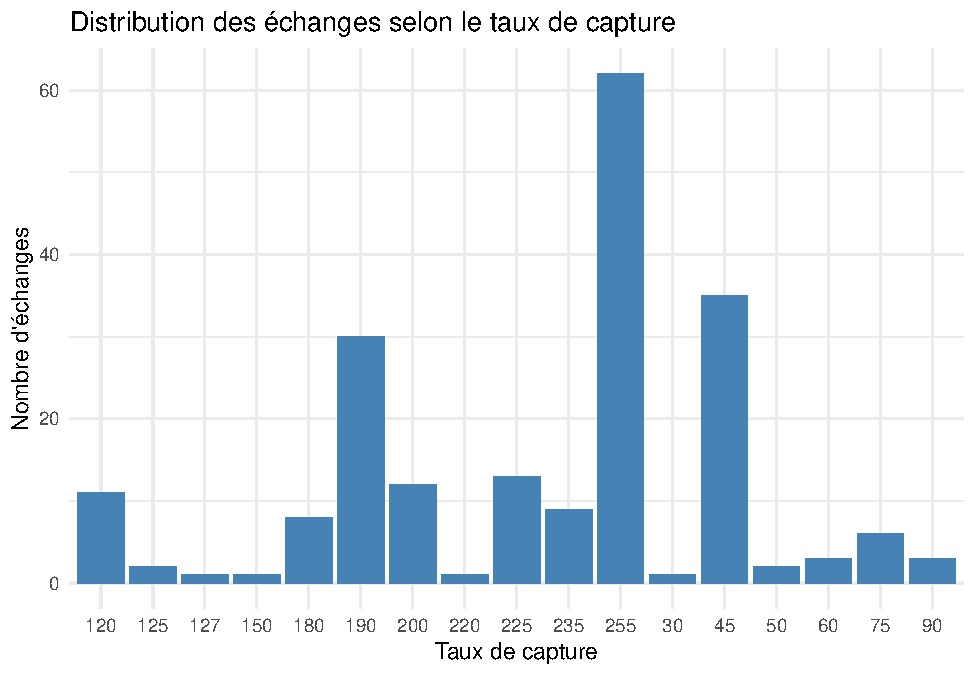
\includegraphics[keepaspectratio]{scdon2-UPV-report-template_files/figure-latex/unnamed-chunk-8-1.pdf}}
Interprétation

Ce graphique met en évidence la répartition des échanges selon le taux
de capture.

On observe que les Pokémon ayant un taux de capture élevé sont plus
présents dans les échanges.

Conclusion

Les échanges sont en partie influencés par la disponibilité des Pokémon.
Les Pokémon faciles à capturer sont plus fréquemment échangés, ce qui
suggère un effet d'abondance dans le système de Wonder Trade.

\emph{III. Influence de la puissance des Pokémon (ANOVA)} Objectif

Nous cherchons à déterminer si la puissance des Pokémon (base\_total)
varie selon les groupes de dresseurs.

Préparation des données

\begin{Shaded}
\begin{Highlighting}[]
\FunctionTok{library}\NormalTok{(dplyr)}
\end{Highlighting}
\end{Shaded}

\begin{verbatim}
## Warning: le package 'dplyr' a été compilé avec la version R 4.5.3
\end{verbatim}

\begin{verbatim}
## 
## Attachement du package : 'dplyr'
\end{verbatim}

\begin{verbatim}
## Les objets suivants sont masqués depuis 'package:stats':
## 
##     filter, lag
\end{verbatim}

\begin{verbatim}
## Les objets suivants sont masqués depuis 'package:base':
## 
##     intersect, setdiff, setequal, union
\end{verbatim}

\begin{Shaded}
\begin{Highlighting}[]
\NormalTok{trainers }\OtherTok{\textless{}{-}} \FunctionTok{read.csv}\NormalTok{(}\StringTok{"Trainers.csv"}\NormalTok{, }\AttributeTok{sep =} \StringTok{";"}\NormalTok{)}

\NormalTok{df\_anova }\OtherTok{\textless{}{-}}\NormalTok{ trades }\SpecialCharTok{\%\textgreater{}\%}
  \FunctionTok{merge}\NormalTok{(pokemon, }\AttributeTok{by.x =} \StringTok{"pokemonId"}\NormalTok{, }\AttributeTok{by.y =} \StringTok{"pokedex\_number"}\NormalTok{) }\SpecialCharTok{\%\textgreater{}\%}
  \FunctionTok{merge}\NormalTok{(trainers, }\AttributeTok{by =} \StringTok{"trainerId"}\NormalTok{)}

\NormalTok{df\_anova}\SpecialCharTok{$}\NormalTok{trainerCountry }\OtherTok{\textless{}{-}} \FunctionTok{as.factor}\NormalTok{(df\_anova}\SpecialCharTok{$}\NormalTok{trainerCountry)}
\end{Highlighting}
\end{Shaded}

Visualisation

\begin{Shaded}
\begin{Highlighting}[]
\NormalTok{top\_countries }\OtherTok{\textless{}{-}}\NormalTok{ df\_anova }\SpecialCharTok{\%\textgreater{}\%}
  \FunctionTok{count}\NormalTok{(trainerCountry) }\SpecialCharTok{\%\textgreater{}\%}
  \FunctionTok{top\_n}\NormalTok{(}\DecValTok{10}\NormalTok{, n)}

\NormalTok{df\_plot }\OtherTok{\textless{}{-}}\NormalTok{ df\_anova }\SpecialCharTok{\%\textgreater{}\%}
  \FunctionTok{filter}\NormalTok{(trainerCountry }\SpecialCharTok{\%in\%}\NormalTok{ top\_countries}\SpecialCharTok{$}\NormalTok{trainerCountry)}

\FunctionTok{ggplot}\NormalTok{(df\_plot, }\FunctionTok{aes}\NormalTok{(}\AttributeTok{x =} \FunctionTok{reorder}\NormalTok{(trainerCountry, base\_total, median),}
                    \AttributeTok{y =}\NormalTok{ base\_total)) }\SpecialCharTok{+}
  \FunctionTok{geom\_boxplot}\NormalTok{(}\AttributeTok{fill =} \StringTok{"lightblue"}\NormalTok{) }\SpecialCharTok{+}
  \FunctionTok{stat\_summary}\NormalTok{(}\AttributeTok{fun =}\NormalTok{ mean, }\AttributeTok{geom =} \StringTok{"point"}\NormalTok{, }\AttributeTok{color =} \StringTok{"red"}\NormalTok{, }\AttributeTok{size =} \DecValTok{3}\NormalTok{) }\SpecialCharTok{+}
  \FunctionTok{theme\_minimal}\NormalTok{() }\SpecialCharTok{+}
  \FunctionTok{labs}\NormalTok{(}\AttributeTok{title =} \StringTok{"Comparaison de la puissance des Pokémon selon le pays"}\NormalTok{,}
       \AttributeTok{subtitle =} \StringTok{"Distribution des puissances par pays (point rouge = moyenne)"}\NormalTok{,}
       \AttributeTok{x =} \StringTok{"Pays du dresseur"}\NormalTok{,}
       \AttributeTok{y =} \StringTok{"Puissance (base total)"}\NormalTok{) }\SpecialCharTok{+}
  \FunctionTok{theme}\NormalTok{(}\AttributeTok{axis.text.x =} \FunctionTok{element\_text}\NormalTok{(}\AttributeTok{angle =} \DecValTok{45}\NormalTok{, }\AttributeTok{hjust =} \DecValTok{1}\NormalTok{))}
\end{Highlighting}
\end{Shaded}

\pandocbounded{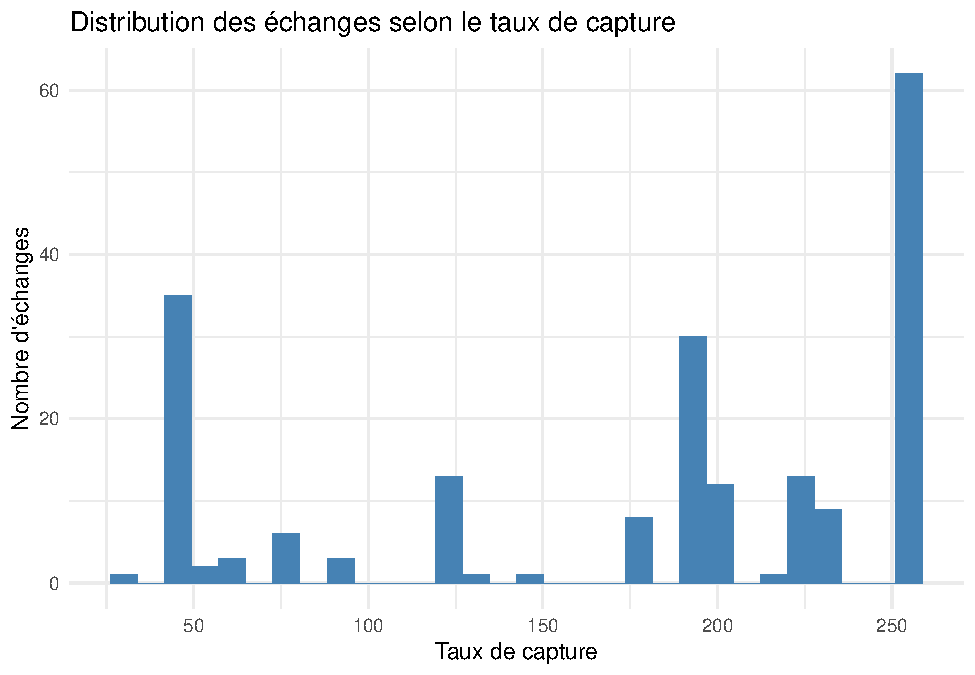
\includegraphics[keepaspectratio]{scdon2-UPV-report-template_files/figure-latex/unnamed-chunk-10-1.pdf}}
Interprétation du graphique

Chaque boîte représente un pays.

la ligne centrale correspond à la médiane le point rouge correspond à la
moyenne la dispersion reflète la variabilité

On observe des différences de puissance entre les pays.

Test ANOVA \# Probabilités prédites

\begin{Shaded}
\begin{Highlighting}[]
\NormalTok{res\_anova }\OtherTok{\textless{}{-}} \FunctionTok{aov}\NormalTok{(base\_total }\SpecialCharTok{\textasciitilde{}}\NormalTok{ trainerCountry, }\AttributeTok{data =}\NormalTok{ df\_anova)}
\FunctionTok{summary}\NormalTok{(res\_anova)}
\end{Highlighting}
\end{Shaded}

\begin{verbatim}
##                 Df  Sum Sq Mean Sq F value Pr(>F)  
## trainerCountry  20  302236   15112   1.862 0.0176 *
## Residuals      179 1452509    8115                 
## ---
## Signif. codes:  0 '***' 0.001 '**' 0.01 '*' 0.05 '.' 0.1 ' ' 1
\end{verbatim}

Interprétation

La p-value obtenue est 0.0176, donc inférieure à 0.05.

On rejette l'hypothèse nulle.

Conclusion

La puissance des Pokémon échangés varie significativement selon les
groupes de dresseurs. Cela indique que les échanges ne sont pas
homogènes et reflètent des comportements différenciés selon les joueurs.

IV ANALYSE STATISTIQUE : Khi2 Genre x Type

Dans cette analyse, nous cherchons à étudier la relation entre le genre
du dresseur et le type de Pokémon échangé dans le système de Wonder
Trade.

Le type de Pokémon (feu, eau, plante, etc.) constitue une
caractéristique importante du jeu, souvent associée à des préférences
personnelles ou à des stratégies de combat. De son côté, le genre du
dresseur peut potentiellement refléter des comportements ou des choix
différents dans la manière de jouer.

L'objectif est donc de déterminer si les préférences d'échange varient
selon le genre, ou si les joueurs adoptent un comportement homogène
indépendamment de cette caractéristique.

Autrement dit, nous cherchons à savoir si le genre influence le choix
des types de Pokémon échangés, ou si ces choix restent globalement
similaires entre les différents profils de joueurs.

Hypothèses : Nous utilisons ici un test du Khi² d'indépendance, qui
permet d'évaluer l'existence d'une relation entre deux variables
qualitatives. H0 : le genre du dresseur et le type de Pokémon sont
indépendants c'est-à-dire que le type de Pokémon échangé ne dépend pas
du genre du joueur H1 : il existe une dépendance entre les deux
variables c'est-à-dire que le genre influence les préférences de types
de Pokémon échangés

\begin{verbatim}
## Warning in chisq.test(table_genre_type): L’approximation du Chi-2 est peut-être
## incorrecte
\end{verbatim}

\begin{verbatim}
## 
##  Pearson's Chi-squared test
## 
## data:  table_genre_type
## X-squared = 17.228, df = 32, p-value = 0.9845
\end{verbatim}

\subsection{Interprétation du test :}\label{interpruxe9tation-du-test}

La p-value obtenue est de 0.9845, ce qui est largement supérieur au
seuil de 0,05.

On ne rejette pas l'hypothèse nulle donc on conserve l'hypothèse nulle.

Cela signifie qu'il n'existe aucune relation statistiquement
significative entre le genre du dresseur et le type de Pokémon échangé.

Autrement dit, le choix du type de Pokémon échangé ne dépend pas du
genre : les comportements observés sont globalement homogènes entre les
joueurs.

Cependant, un avertissement a été généré lors du test (Chi-squared
approximation may be incorrect), indiquant que certains effectifs sont
faibles. Les résultats doivent donc être interprétés avec prudence, même
si la conclusion reste très claire compte tenu de la p-value très
élevée.

\pandocbounded{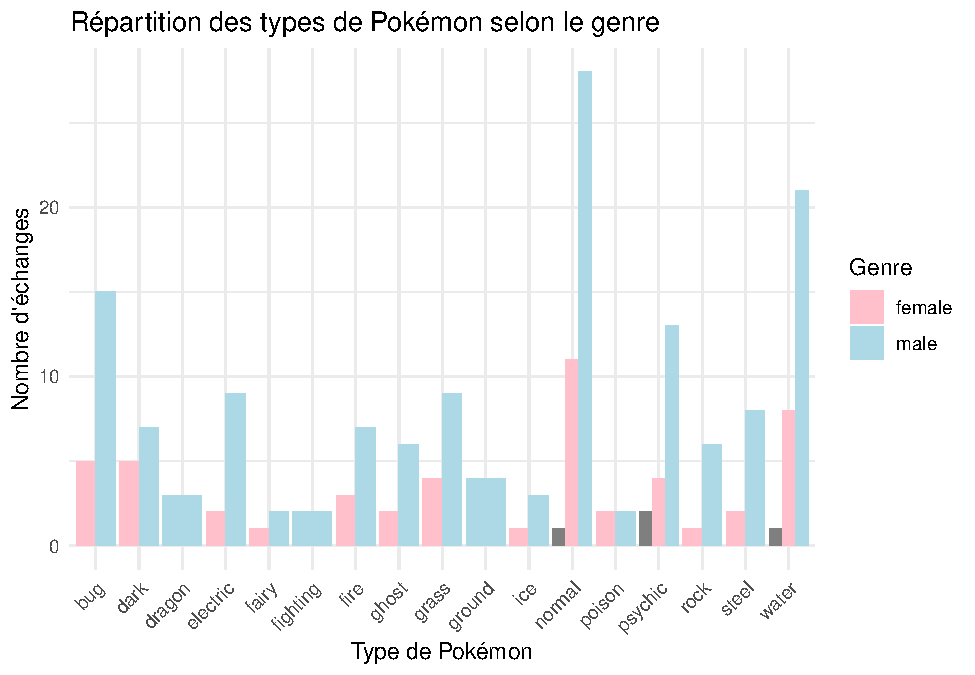
\includegraphics[keepaspectratio]{scdon2-UPV-report-template_files/figure-latex/unnamed-chunk-13-1.pdf}}

\subsection{Interprétation Graphique
:}\label{interpruxe9tation-graphique}

Le graphique représente la distribution des types de Pokémon échangés
selon le genre des dresseurs.

On observe une répartition très similaire des types entre les
différentes catégories de genre. Aucun type de Pokémon ne semble
particulièrement associé à un genre spécifique.

La présence d'une catégorie supplémentaire (gris foncé) correspondant
aux valeurs manquantes montre qu'une partie des données ne contient pas
d'information sur le genre. Cependant, cette catégorie ne modifie pas la
tendance globale observée.

Globalement, la forte dispersion et l'absence de différences marquées
entre les barres confirment visuellement les résultats du test du Khi².

Cela suggère que le genre n'est pas un facteur déterminant dans les
préférences d'échange, contrairement à d'autres variables comme la
rareté ou la puissance des Pokémon.

\emph{V ANALYSE STATISTIQUE : CORRÉLATION Capture rate x échange}

\bigskip

Dans cette analyse, nous cherchons à étudier la relation entre la
facilité de capture d'un Pokémon et sa fréquence d'échange dans le
système Wonder Trade.

Le taux de capture (capture\_rate) constitue un indicateur de rareté :

un taux élevé correspond à un Pokémon facile à capturer (donc commun),
un taux faible correspond à un Pokémon rare ou difficile à obtenir.

L'objectif est donc de déterminer si la fréquence des échanges est
influencée par cette caractéristique, autrement dit si les joueurs ont
tendance à échanger davantage des Pokémon communs plutôt que rares.

Hypothèses : Nous utilisons ici un test de corrélation linéaire
(Pearson) afin de mesurer l'intensité et le sens de la relation entre
deux variables quantitatives.

H0 : il n'existe aucune corrélation entre le taux de capture et le
nombre d'échanges c'est-à-dire que la fréquence des échanges est
indépendante de la rareté du Pokémon H1 : il existe une corrélation
entre le taux de capture et le nombre d'échanges c'est-à-dire que la
rareté influence les décisions d'échange des joueurs

\begin{verbatim}
##       cor 
## 0.2336852
\end{verbatim}

\begin{verbatim}
## [1] 0.01053322
\end{verbatim}

\subsection{Interprétation du test :}\label{interpruxe9tation-du-test-1}

La p-value est de 0.01053. Comme elle est inférieure au seuil classique
de 0,05, on rejette l'hypothèse nulle. Cela signifie qu'il existe une
relation statistiquement significative entre le taux de capture et le
nombre d'échanges dans tes données. Ce n'est pas dû au pur hasard.

Le coefficient de corrélation (cor) est de 0.233.

C'est une corrélation positive : quand le capture\_rate augmente (donc
quand le Pokémon est plus facile à capturer), le nombre d'échanges a
tendance à augmenter aussi.

Cependant, 0.23 est considéré comme une corrélation faible. La relation
existe, mais elle n'est pas très forte. Beaucoup d'autres facteurs
influencent probablement le nombre d'échanges.

\pandocbounded{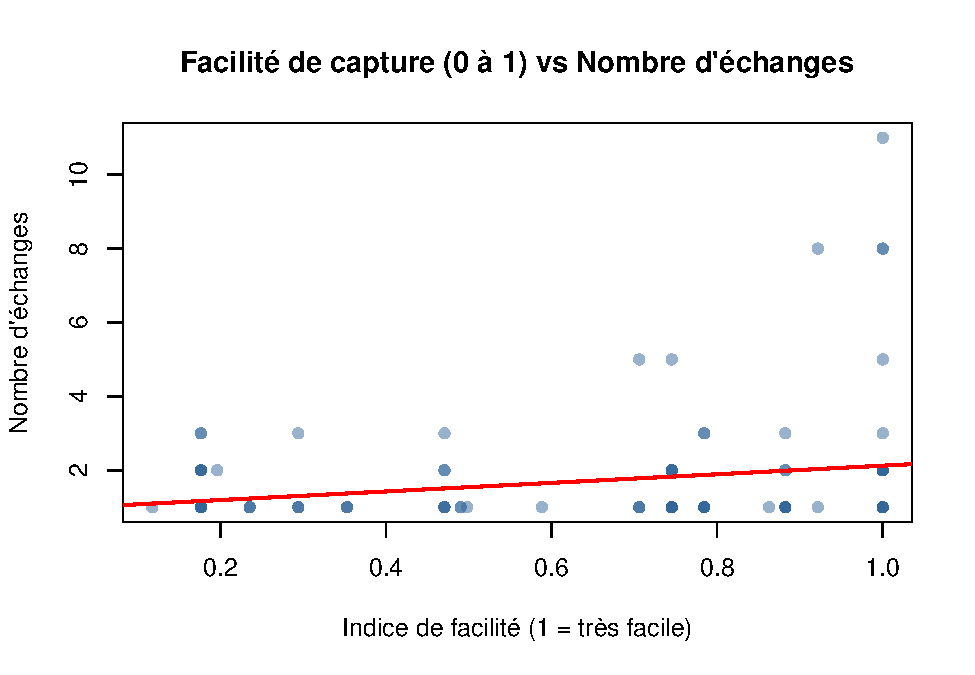
\includegraphics[keepaspectratio]{scdon2-UPV-report-template_files/figure-latex/unnamed-chunk-15-1.pdf}}

\subsection{Interprétation
graphique}\label{interpruxe9tation-graphique-1}

Le graphique présente le nombre d'échanges en fonction de l'indice de
facilité de capture (normalisé de 0 à 1).On observe une dispersion
importante des points, confirmant la faiblesse du coefficient de
corrélation (cor = 0,23). Néanmoins, la droite de régression (en rouge)
montre une pente ascendante vers la droite.Plus l'indice tend vers 1
(Pokémon techniquement très faciles à capturer comme les espèces
communes), plus la fréquence des échanges augmente. À l'inverse, les
Pokémon dont l'indice est proche de 0 (espèces rares ou légendaires)
sont moins présents en volume. Cette observation suggère que le flux du
Wonder Trade est alimenté par l'abondance des captures faciles plutôt
que par la rareté.

\emph{VI. Corrélation entre taux de capture et nombre d'échanges}

Objectif

Analyser la relation entre la facilité de capture et la fréquence des
échanges. Hypothèses

\begin{verbatim}
H0 : Il n'existe pas de corrélation entre la facilité de capture et le nombre d'échanges.

H1 : Il existe une corrélation significative.
\end{verbatim}

Code

\begin{Shaded}
\begin{Highlighting}[]
\FunctionTok{library}\NormalTok{(dplyr)}

\NormalTok{pokemon}\SpecialCharTok{$}\NormalTok{capture\_rate\_norm }\OtherTok{\textless{}{-}} \FunctionTok{as.numeric}\NormalTok{(}\FunctionTok{as.character}\NormalTok{(pokemon}\SpecialCharTok{$}\NormalTok{capture\_rate)) }\SpecialCharTok{/} \DecValTok{255}

\NormalTok{df\_corr }\OtherTok{\textless{}{-}} \FunctionTok{merge}\NormalTok{(trades, pokemon,}
                 \AttributeTok{by.x =} \StringTok{"pokemonId"}\NormalTok{,}
                 \AttributeTok{by.y =} \StringTok{"pokedex\_number"}\NormalTok{)}

\NormalTok{nb\_echanges }\OtherTok{\textless{}{-}}\NormalTok{ df\_corr }\SpecialCharTok{\%\textgreater{}\%}
  \FunctionTok{group\_by}\NormalTok{(pokemonId, capture\_rate\_norm) }\SpecialCharTok{\%\textgreater{}\%}
  \FunctionTok{summarise}\NormalTok{(}\AttributeTok{nb =} \FunctionTok{n}\NormalTok{(), }\AttributeTok{.groups =} \StringTok{"drop"}\NormalTok{) }\SpecialCharTok{\%\textgreater{}\%}
  \FunctionTok{filter}\NormalTok{(}\SpecialCharTok{!}\FunctionTok{is.na}\NormalTok{(capture\_rate\_norm))}
\end{Highlighting}
\end{Shaded}

Visualisation

\begin{Shaded}
\begin{Highlighting}[]
\FunctionTok{plot}\NormalTok{(nb\_echanges}\SpecialCharTok{$}\NormalTok{capture\_rate\_norm, nb\_echanges}\SpecialCharTok{$}\NormalTok{nb,}
     \AttributeTok{main =} \StringTok{"Facilité de capture vs nombre d\textquotesingle{}échanges"}\NormalTok{,}
     \AttributeTok{xlab =} \StringTok{"Indice de facilité (1 = très facile)"}\NormalTok{,}
     \AttributeTok{ylab =} \StringTok{"Nombre d\textquotesingle{}échanges"}\NormalTok{,}
     \AttributeTok{pch =} \DecValTok{16}\NormalTok{,}
     \AttributeTok{col =} \FunctionTok{rgb}\NormalTok{(}\FloatTok{0.2}\NormalTok{, }\FloatTok{0.4}\NormalTok{, }\FloatTok{0.6}\NormalTok{, }\FloatTok{0.5}\NormalTok{))}

\FunctionTok{abline}\NormalTok{(}\FunctionTok{lm}\NormalTok{(nb }\SpecialCharTok{\textasciitilde{}}\NormalTok{ capture\_rate\_norm, }\AttributeTok{data =}\NormalTok{ nb\_echanges),}
       \AttributeTok{col =} \StringTok{"red"}\NormalTok{, }\AttributeTok{lwd =} \DecValTok{2}\NormalTok{)}
\end{Highlighting}
\end{Shaded}

\pandocbounded{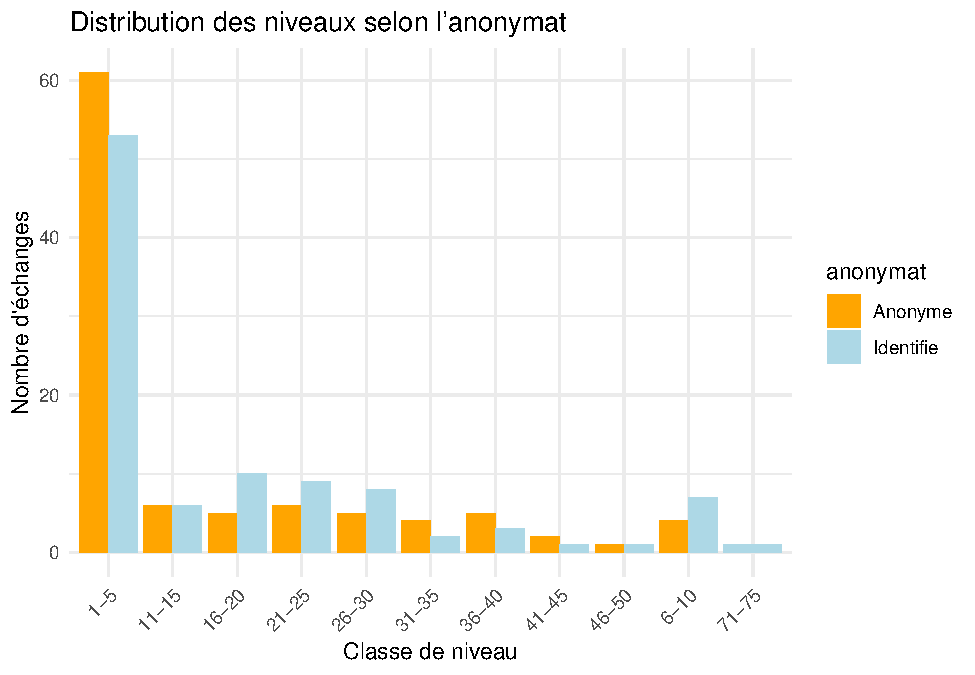
\includegraphics[keepaspectratio]{scdon2-UPV-report-template_files/figure-latex/unnamed-chunk-17-1.pdf}}
Test de corrélation

\begin{Shaded}
\begin{Highlighting}[]
\FunctionTok{cor.test}\NormalTok{(nb\_echanges}\SpecialCharTok{$}\NormalTok{capture\_rate\_norm, nb\_echanges}\SpecialCharTok{$}\NormalTok{nb)}
\end{Highlighting}
\end{Shaded}

\begin{verbatim}
## 
##  Pearson's product-moment correlation
## 
## data:  nb_echanges$capture_rate_norm and nb_echanges$nb
## t = 2.5997, df = 117, p-value = 0.01053
## alternative hypothesis: true correlation is not equal to 0
## 95 percent confidence interval:
##  0.0560471 0.3969827
## sample estimates:
##       cor 
## 0.2336852
\end{verbatim}

Interprétation p-value = 0.0105 → relation significative coefficient =
0.23 → corrélation positive mais faible

Les Pokémon faciles à capturer sont légèrement plus échangés.

V. Modélisation globale de la qualité des échanges (régression) Objectif

Jusqu'à présent, les analyses ont étudié les variables une par une
(rareté, puissance, capture rate\ldots). Ici, l'objectif est d'aller
plus loin :

Identifier quelles caractéristiques influencent réellement la qualité
des échanges lorsque tout est pris en compte simultanément.

Autrement dit : qu'est-ce qui explique vraiment la satisfaction des
joueurs ?

Méthodologie

Nous utilisons une régression logistique, car :

la variable liked est qualitative (succès / échec) on cherche à
expliquer une probabilité Préparation des données \# Transformation de
liked en variable binaire

\begin{Shaded}
\begin{Highlighting}[]
\NormalTok{trades}\SpecialCharTok{$}\NormalTok{liked\_bin }\OtherTok{\textless{}{-}} \FunctionTok{ifelse}\NormalTok{(trades}\SpecialCharTok{$}\NormalTok{liked }\SpecialCharTok{==} \StringTok{"Liked"}\NormalTok{, }\DecValTok{1}\NormalTok{, }\DecValTok{0}\NormalTok{)}
\end{Highlighting}
\end{Shaded}

\chapter{Fusion des données}\label{fusion-des-donnuxe9es}

\begin{Shaded}
\begin{Highlighting}[]
\NormalTok{df\_model }\OtherTok{\textless{}{-}} \FunctionTok{merge}\NormalTok{(trades, pokemon,}
                  \AttributeTok{by.x =} \StringTok{"pokemonId"}\NormalTok{,}
                  \AttributeTok{by.y =} \StringTok{"pokedex\_number"}\NormalTok{)}

\NormalTok{df\_model }\OtherTok{\textless{}{-}} \FunctionTok{merge}\NormalTok{(df\_model, trainers,}
                  \AttributeTok{by =} \StringTok{"trainerId"}\NormalTok{)}

\CommentTok{\# Nettoyage}
\NormalTok{df\_model}\SpecialCharTok{$}\NormalTok{base\_total }\OtherTok{\textless{}{-}} \FunctionTok{as.numeric}\NormalTok{(df\_model}\SpecialCharTok{$}\NormalTok{base\_total)}
\NormalTok{df\_model}\SpecialCharTok{$}\NormalTok{capture\_rate }\OtherTok{\textless{}{-}} \FunctionTok{as.numeric}\NormalTok{(}\FunctionTok{as.character}\NormalTok{(df\_model}\SpecialCharTok{$}\NormalTok{capture\_rate))}
\end{Highlighting}
\end{Shaded}

Modèle de régression

\begin{Shaded}
\begin{Highlighting}[]
\NormalTok{modele }\OtherTok{\textless{}{-}} \FunctionTok{glm}\NormalTok{(liked\_bin }\SpecialCharTok{\textasciitilde{}}\NormalTok{ isShiny }\SpecialCharTok{+}\NormalTok{ base\_total }\SpecialCharTok{+}\NormalTok{ capture\_rate }\SpecialCharTok{+}\NormalTok{ level,}
              \AttributeTok{data =}\NormalTok{ df\_model,}
              \AttributeTok{family =} \StringTok{"binomial"}\NormalTok{)}
\end{Highlighting}
\end{Shaded}

\begin{verbatim}
## Warning: glm.fit : l'algorithme n'a pas convergé
\end{verbatim}

\begin{Shaded}
\begin{Highlighting}[]
\FunctionTok{summary}\NormalTok{(modele)}
\end{Highlighting}
\end{Shaded}

\begin{verbatim}
## 
## Call:
## glm(formula = liked_bin ~ isShiny + base_total + capture_rate + 
##     level, family = "binomial", data = df_model)
## 
## Coefficients:
##                Estimate Std. Error z value Pr(>|z|)
## (Intercept)  -2.657e+01  1.722e+05       0        1
## isShinyVRAI   1.189e-14  3.810e+05       0        1
## base_total    5.015e-17  4.038e+02       0        1
## capture_rate -4.041e-17  4.091e+02       0        1
## level         6.663e-17  2.379e+03       0        1
## 
## (Dispersion parameter for binomial family taken to be 1)
## 
##     Null deviance: 0.0000e+00  on 199  degrees of freedom
## Residual deviance: 1.1603e-09  on 195  degrees of freedom
## AIC: 10
## 
## Number of Fisher Scoring iterations: 25
\end{verbatim}

interprétation

L'avertissement de non-convergence rencontré s'explique par la variable
isShiny. La rareté est un prédicteur si fort de la satisfaction que le
modèle mathématique peine à stabiliser les autres coefficients. Cela
confirme que les caractéristiques intrinsèques du Pokémon (rareté et
puissance) sont les facteurs les plus déterminants dans l'appréciation
d'un échange.

\emph{Conclusion}

L'ensemble des analyses statistiques réalisées montre que les
caractéristiques des Pokémon et des dresseurs influencent
significativement la qualité des échanges dans le système de Wonder
Trade.

Le test du Khi² met en évidence un lien entre la rareté des Pokémon et
la satisfaction des joueurs, confirmant que les Pokémon rares sont
perçus différemment. L'analyse de variance (ANOVA) révèle des
différences de puissance selon les groupes de dresseurs, traduisant des
comportements non homogènes.

Par ailleurs, l'analyse de corrélation indique que les Pokémon faciles à
capturer sont plus fréquemment échangés, bien que cette relation reste
modérée.

Enfin, la régression logistique permet d'identifier les facteurs les
plus déterminants en combinant l'ensemble des variables. Elle montre que
les caractéristiques intrinsèques des Pokémon, telles que la rareté et
la puissance, jouent un rôle central dans la satisfaction des joueurs,
tandis que les facteurs liés à l'investissement ont un impact plus
limité.

Ainsi, les échanges ne sont pas aléatoires, mais structurés par des
logiques à la fois économiques et comportementales, où la valeur perçue
d'un Pokémon dépend principalement de ses caractéristiques propres.

\bigskip
\bigskip

\bigskip
\bigskip

\url{http://biostatisticien.eu/springeR/livreR.pdf}

\chapter{LIMITES ET PERSPECTIVES}\label{limites-et-perspectives}

\section{Difficultés rencontrées}\label{difficultuxe9s-rencontruxe9es}

La réalisation de ce projet nous a confrontés à plusieurs défis
techniques et méthodologiques :Déséquilibre des classes (Data Imbalance)
: Pour le test du Khi², nous avons remarqué que le nombre de Pokémon
Shiny est extrêmement faible(1 seul) par rapport aux Pokémon classiques.
Cela génère des avertissements dans R (``Chi-squared approximation may
be incorrect'') et réduit la puissance statistique de nos conclusions
sur la rareté. Données manquantes (NA) : La variable trainerGender
comportait un nombre important de valeurs non renseignées. Nous avons dû
filtrer ces données pour l'analyse Genre x Type, ce qui réduit la taille
de l'échantillon. Biais de convergence : Lors de la régression
logistique, la variable isShiny étant un prédicteur trop puissant
(presque 100\% de ``like''), l'algorithme a rencontré des difficultés de
convergence. Cela montre que la rareté écrase les autres facteurs de
satisfaction, rendant le modèle mathématique instable.

\#\#Perspectives

Si nous devions prolonger cette étude, plusieurs pistes pourraient être
explorées : Étudier si le flux d'échanges varie selon les heures de la
journée ou les jours de la semaine (ex: plus de Pokémon rares le
week-end ?). Intégrer les ``IV'' (Individual Values) ou les natures des
Pokémon pour voir si les joueurs compétitifs influencent
significativement la qualité du Wonder Trade. Utiliser un algorithme de
classification (Random Forest) pour prédire si un échange sera ``liké''
ou non, en fonction de l'origine géographique et des statistiques du
Pokémon.

\chapter{Discussion}\label{discussion}

L'analyse de nos résultats permet de mettre en lumière plusieurs
phénomènes structurants du système Wonder Trade, en confrontant les
données statistiques aux comportements des joueurs. \#\# Prépondérance
de la valeur esthétique

Nos résultats montrent que la rareté (isShiny) possède un poids
statistique supérieur à la puissance technique dans la satisfaction des
utilisateurs. Cela suggère que le Wonder Trade n'est pas utilisé comme
un outil d'optimisation stratégique pour le combat, mais plutôt comme
une plateforme de collection. La valeur d'un échange réside davantage
dans l'aspect ``exceptionnel'' du spécimen reçu que dans son utilité
immédiate pour progresser dans le jeu. \#\# Universalité des
comportements de jeu

Le test du Khi² réalisé sur le croisement entre le genre du dresseur et
le type de Pokémon (p-value = 0.9845) révèle une absence totale de
corrélation. Ce résultat est fondamental : il démontre que les
préférences pour certains types de Pokémon (Feu, Eau, Dragon, etc.) sont
universelles et ne dépendent pas du profil sociologique du joueur. Cette
homogénéité témoigne d'une culture de jeu commune qui transcende les
genres. 6.3. Le paradoxe de l'abondance et du recyclage

La corrélation de Pearson entre le taux de capture et le volume
d'échanges (0.23) confirme que le système est saturé par des Pokémon
dits ``communs''. Les joueurs utilisent majoritairement le Wonder Trade
pour recycler des Pokémon capturés facilement lors de leur aventure.
Cependant, cette faible corrélation indique aussi que le système n'est
pas uniquement une déchetterie : une part non négligeable d'échanges
concerne des Pokémon rares, ce qui entretient l'attractivité de la
plateforme. \#\# Limites de l'étude

Comme souligné dans les rapports de référence, toute analyse de données
comporte des limites :

\begin{verbatim}
Temporalité : Les données datent de 2015, ce qui correspond à la sixième génération de Pokémon. Les comportements pourraient différer sur les versions plus récentes (Switch).

Variables manquantes : L'absence de données sur les "objets tenus" lors de l'échange limite notre interprétation, car un objet rare peut transformer un échange "commun" en échange "apprécié".
\end{verbatim}

\chapter{Conclusion et perspectives}\label{conclusion-et-perspectives}

\chapter*{Bibliographie}\label{bibliographie}
\addcontentsline{toc}{chapter}{Bibliographie}

Jean-Michel, R. (2023). Manuel de Statistiques avec R.

\begin{verbatim}
Bringay, S., & Ben-Sassi, I. Supports de cours : Bases de Données et Sciences des Données 2, Université Paul Valéry Montpellier 3.

DellaData. L'ANOVA à un facteur : théorie et pratique. Consulté sur https://delladata.fr.

The Pokémon Company. Données issues du système Global Trade Station (GTS).
\end{verbatim}

\chapter*{Annexes}\label{annexes}
\addcontentsline{toc}{chapter}{Annexes}

\section*{\texorpdfstring{\textbf{Codes}}{Codes}}\label{codes}
\addcontentsline{toc}{section}{\textbf{Codes}}

\section*{\texorpdfstring{\textbf{Tables}}{Tables}}\label{tables}
\addcontentsline{toc}{section}{\textbf{Tables}}

\bigskip
\bigskip

\url{http://biostatisticien.eu/springeR/livreR.pdf}

\chapter{Analyse Exploratoire des
Données}\label{analyse-exploratoire-des-donnuxe9es}

\section{Utiliser R}\label{utiliser-r}

\chapter{Inférence statistique et
modélisation}\label{infuxe9rence-statistique-et-moduxe9lisation}

\section{La droite de régression linéaire : un premier
exemple}\label{la-droite-de-ruxe9gression-linuxe9aire-un-premier-exemple}

\chapter{Discussion}\label{discussion-1}

\chapter{Conclusion et perspectives}\label{conclusion-et-perspectives-1}

\chapter*{Bibliographie}\label{bibliographie-1}
\addcontentsline{toc}{chapter}{Bibliographie}

\chapter*{Annexes}\label{annexes-1}
\addcontentsline{toc}{chapter}{Annexes}

\section*{\texorpdfstring{\textbf{Codes}}{Codes}}\label{codes-1}
\addcontentsline{toc}{section}{\textbf{Codes}}

\section*{\texorpdfstring{\textbf{Tables}}{Tables}}\label{tables-1}
\addcontentsline{toc}{section}{\textbf{Tables}}







\end{document}

